\documentclass[review,3p,10pt]{elsarticle}

%\usepackage{natbib}

\biboptions{sort&compress}

%\usepackage[numbers,sort&compress]{natbib}
%\usepackage[colorlinks=true,linkcolor=black, citecolor=blue, urlcolor=blue]{hyperref}

\usepackage{amssymb}
\usepackage{amsmath}
\usepackage{cases}
\usepackage{epstopdf}
\interdisplaylinepenalty=500
%\usepackage[caption=false,font=footnotesize]{subfig}
\usepackage{fixltx2e}
\usepackage{mathtools}
\usepackage{array}
\usepackage{bm}
\usepackage{multirow}
\usepackage{color}
\usepackage{algorithm}
\usepackage{algorithmic}
\usepackage{amsthm}
\usepackage{mathrsfs}
\usepackage{amssymb}
\newtheorem{theorem}{Theorem}
\newtheorem{lemma}{Lemma}
\newtheorem{assumption}{Assumption}
\newtheorem{proposition}{Proposition}
\newtheorem{remark}{Remark}
\usepackage{lineno}
%\linenumbers

\DeclarePairedDelimiter\ceil{\lceil}{\rceil}
\DeclarePairedDelimiter\floor{\lfloor}{\rfloor}


\usepackage{url}
\def\UrlBreaks{\do\/\do-}

\newcommand{\tabincell}[2]{\renewcommand\arraystretch{0.8}\begin{tabular}{@{}#1@{}}#2\end{tabular}}

%\journal{Applied Energy}
%\journal{International Journal of Hydrogen Energy}
\journal{arXiv.org}


\begin{document}
\begin{frontmatter}

%\title{Flexibility Assessment and Aggregation of Alkaline Electrolyzers under Dynamic Thermal and HTO Impurity Constraints for Renewable Power-to-Hydrogen Energy Management}
\title{Dynamic Operation and Control
	of a Multi-Stack Alkaline Water
	 Electrolysis System with Shared Gas Separators and Lye Circulation:\\ A Model-Based Study}


\author[label1]{Yiwei~Qiu}
\author[label1]{Jiatong~Li}
\author[label1]{Yangjun~Zeng}
\author[label1]{Yi~Zhou\corref{cor1}}
\ead{yizhou3230@scu.edu.cn}
\author[label1]{Shi~Chen}
\author[label1]{Xiaoyan~Qiu}
\author[label1]{Buxiang~Zhou}
\author[label2]{Ge~He}
\author[label2]{Xu~Ji}
\author[label3]{Wenying~Li}

\address[label1]{College of Electrical Engineering, Sichuan University, Chengdu, 610065, China}
\cortext[cor1]{Corresponding author}
\address[label2]{School of Chemical Engineering, Sichuan University, Chengdu, 610065, China}
\address[label3]{Sichuan Tsinghua Energy Internet Research Institute, Chengdu, 610213, China}

\begin{abstract}
   An emerging approach for large-scale hydrogen production using renewable energy is to integrate multiple alkaline water electrolysis (AWE) stacks into a single balance of plant (BoP) system, sharing components such as gas-lye separation and lye circulation. This configuration, termed the $N$-in-1 AWE system, packs $N$ stacks into a modular system, reducing land requirements, the complexity of plant topology, and overall capital costs. However, the coupling of these stacks through the shared BoP introduces challenges in dynamic operation under varying energy inputs, making their performance unclear compared to traditional 1-in-1 systems. To address this, we develop a state-space model of the $N$-in-1 AWE system, capturing the dynamic behaviors of lye circulation, temperature, and HTO impurity, and their impact on energy conversion efficiency. We then propose a nonlinear model predictive controller (NMPC) to coordinately optimize inter-stack electrolytic current distribution, lye flow, and cooling, enabling the system to dynamically track varying load commands while maximizing efficiency, stabilizing temperature, and limiting HTO impurity accumulation. Simulation studies on a $4,000$ Nm$^3$/h-rated 4-in-1 system verify the proposed controller under dynamic operation. Comparison with 4 independent 1-in-1 systems reveals that, with proper control, the $N$-in-1 configuration offers comparable flexibility in accommodating real-world wind power inputs. The average differences in the root-mean-square errors (RMSEs) for load-tracking and stack temperature stabilization, and specific energy consumption are below $0.014$ MW, $2.356$ K, and $0.003$ kWh/Nm$^3$.
\end{abstract}

\begin{keyword}
    alkaline water electrolysis %(AEL)
    %\sep  advanced process control %(APC)
    \sep  nonlinear model predictive control %(NMPC)
    \sep  balance of plant (BoP)
    \sep  renewable power to hydrogen
\end{keyword}

\end{frontmatter}

\section{Introduction}
\label{sec:intro}

\subsection{Motivation}
\label{sec:motivation}

Water electrolysis for hydrogen production has emerged as a crucial pathway for renewable energy utilization and low-carbon energy transformation, with rapid scaling worldwide \cite{hosseini2022hydrogen}. According to the IEA, the global installed capacity of hydrogen electrolyzers reached 1.4 GW in 2023, doubling from 2022 levels. %Furthermore,
Many countries have incorporated renewable power-to-hydrogen (ReP2H) into their strategic plans, targeting 520 GW of installed capacity by 2030 \cite{IEA2024Global}. Among various hydrogen production technologies, alkaline water electrolysis (AWE) stands out for its maturity, large capacity, long lifespan, and low cost, making it a preferred choice in many ReP2H projects \cite{emam2024review}.

Although the capacity of a single AWE has increased from 1,000 Nm$^3$/h (5 MW) in 2020 to 3,000 Nm$^3$/h (15 MW) today \cite{emam2024review}, the scale remains relatively limited for large-scale applications. Due to the capacity constraints of a single electrolyzer, hydrogen plants often consist of dozens to hundreds of electrolyzers, leading to large land requirements, complex topologies, and high investment costs \cite{emam2024review}. The acquisition and installation costs of electrolyzers, as well as land and infrastructure investments, are critical considerations in practices \cite{lange2024modularization,niblett2024review}. To reduce costs and improve the economic viability of green hydrogen, shared balance-of-plant (BoP) designs have emerged as a technological route for scaling up AWE systems \cite{lange2024modularization,niblett2024review,chi2024elevating,zhang2024optimizing,yang2022application,rizwan2021design,chen2024enhancing,shi2023plant}.

A typical AWE system consists of an electrolysis stack and a set of BoP system, which includes lye-gas separation, cooling, and lye circulation subsystems, and pumps, valves, instrumentation, and control systems, often integrated as a skid-mounted unit  \cite{emam2024review,niblett2024review}. This is referred to as a \emph{1-in-1} system. However, in large hydrogen plants with many electrolyzers, adopting a 1-in-1 configuration results in excessive land use, complex topologies, and elevated costs. To address these issues, some projects employ \emph{N-in-1} configurations (also referred to as \emph{multi-electrolyzer} systems \cite{liang2024large,li2023exploration},) wherein multiple stacks share a single BoP system, thereby reducing complexity and cost \cite{niblett2024review}.

Engineering practice indicates that replacing a 1-in-1 configuration with a 2-in-1 system can reduce costs by 25\% and land and utility requirements by 45\%, while a 4-in-1 system can achieve savings of 35\% and 55\%, respectively \cite{yang2022application}. Consequently, many large ReP2H projects adopt $N$-in-1 configurations. For example, the \emph{Baofeng Energy Green Hydrogen Development Project} and \emph{Songwon Hydrogen Energy Industrial Park Project} utilize 2-in-1 systems as the basic production unit \cite{meng2024advantages,zhangalkaline}, while the \emph{Sinopec Kuqa Green Hydrogen Demonstration Project} and the \emph{Da'an Wind and Solar Green Hydrogen Synthesis Ammonia Integration Demonstration Project} adopt 4-in-1 configurations to enable larger-scale plant designs \cite{zhangalkaline,zhai2024review}.

However, compared to 1-in-1 systems, $N$-in-1 configurations introduce greater operational complexity due to coupling between stacks through the shared BoP system.
This coupling affects temperature regulation and HTO impurity control, %increasing the complexity of operational management and 
potentially limiting flexibility under varying power inputs \cite{rizwan2021design}. Existing research on the dynamic operation of AWE systems, however, %, including efficiency optimization, temperature stabilization, and HTO impurity suppression,
predominantly focuses on 1-in-1 systems, while studies addressing $N$-in-1 configurations are limited; see Section \ref{sec:review} for literature review. Consequently, two key issues arise in engineering applications:

\begin{enumerate}
  \item How do $N$-in-1 systems compare to 1-in-1 systems in terms of adaptability to variable power inputs, such as load flexibility and energy conversion efficiency? Does the capital cost saved in deploying $N$-in-1 systems come at the expense of operational flexibility?

  \item How can controllers for $N$-in-1 AWE systems be designed to match the performance of 1-in-1 systems, minimizing potential losses in flexibility due to increased complexity?
\end{enumerate}

To address these questions, this study develops a state-space model for $N$-in-1 AWE systems, designs controllers, and evaluates performance metrics. Given the lack of experimental platforms for laboratory-scale $N$-in-1 systems and the challenges of conducting experiments on industry-scale systems (20--40 MW or larger,) %as well as the absence of reported experimental data,
this study adopts a simulation approach. %similar to prior $N$-in-1 studies \cite{yang2022application,rizwan2021design,chen2024enhancing,shi2023plant}.
Section \ref{sec:review} summarizes the current research on AWE modeling and control, while Section \ref{sec:contribution} outlines the contributions of this study.

\subsection{Literature Review}
\label{sec:review}

AWE has a long history of application. In recent years, the increasing practices of ReP2H projects have accelerated %academic 
researches on AWE systems, yielding substantial results and insights.

Extensive studies have been conducted on the components of AWE systems. Many researches focus on the stacks, addressing topics such as electrochemical performance \cite{sanchez2018semi,huang2022multiphysics}, degradation \cite{esfandiari2024metal}, flow field \cite{wang2023non}, and the spatial distribution of temperature \cite{zhang2024temperature}, bubbles \cite{cao2024investigation}, and stray currents \cite{qi2023channel,sakas2024influence,dogan2024experimental}. Additional research has examined BoP components, including efficiency analysis and structural design of separators \cite{wang2022experimental,zeng2020experimental,hu2024study}, heat exchangers \cite{rashidi2022progress,jiang2024performance}, pressure loss and energy consumption in lye circulation \cite{qi2023channel}, and compression and purification networks \cite{kang2018optimal}.

Building on these component-level studies, researchers have developed complete AWE system models %incorporating BoP components 
and designed controllers. % to enhance adaptability to fluctuating energy inputs. 
For example, Ulleberg et al. \cite{ulleberg2003modeling} established a classic lumped dynamic model of electrochemical and thermal behavior. David et al. \cite{david2020dynamic} developed a high-order mass transfer model that captures variations in pressure, liquid levels, and flow compositions. Qi et al. \cite{qi2023thermal,qi2023design,qi2021pressure} proposed 1st- to 3rd-order state-space models to describe temperature dynamics and HTO impurity accumulation under dynamic loads, introducing thermal and pressure management methods to improve energy conversion efficiency and load range. 
%Qiu et al. \cite{qiu2024nonlinear} extended these models by introducing an NMPC approach for automatic generation control (AGC) signal tracking.
Chen et al. \cite{cheng2024self} considered the impacts of temperature and pulse rectification on voltage and current efficiencies, proposing an adaptive MPPT strategy to optimize energy conversion efficiency across the full operating range. 
%Shi et al. \cite{shi2023plant} introduced an RTO-PI dual-layer control strategy to suppress HTO impurity violations under dynamic loads. 
Li et al. \cite{li2022active} proposed a comprehensive control framework addressing temperature, pressure, and lye circulation to enhance performance over the full load range. These models have been validated through experiments at various scales (500 W to 3 MW) \cite{li2022study,ding2023experimental,sakas2022dynamic}. Qiu et al. \cite{qiu2023dynamic} further developed an online identification method for heat and mass transfer parameters, enabling real-time model calibration and health diagnostics. % during field operations.
A comprehensive review of AWE modeling and control is provided in \cite{olivier2017low,daoudi2024overview,aguirre2024control}.

\begin{table}[tb]\scriptsize
  \renewcommand{\arraystretch}{1.22}
  \caption{Summary of the latest research related to process modeling and control of AWE systems}\vspace{6pt}
  \label{tab:literature}
  \centering
  \begin{tabular}{ccccccccc}
  \hline \hline
  \multirow{2}{*}{Literature}                   & \multirow{2}{*}{\tabincell{c}{Configuration}}    & \multicolumn{5}{c}{Considered Processes}
                                                & \multirow{2}{*}{Controller}  \\
  \cline{3-7}
                                                & & \tabincell{c}{Load\\control}            & \tabincell{c}{Lye-gas\\ separation} & \tabincell{c}{Lye\\circulation}  & \tabincell{c}{Thermal\\control}   & \tabincell{c}{HTO\\ impurity}                          &    \\                        \hline
  \tabincell{c}{Qi et al. 2023 \cite{qi2023thermal,qi2023design}}       & 1-in-1   & $\times$      & \checkmark          & \checkmark        & \checkmark  & $\times$ & MPC/PID \\
  \tabincell{c}{Qi et al. 2021 \cite{qi2021pressure}}                   & 1-in-1   & $\times$    & \checkmark          & \checkmark        & $\times$  & \checkmark  & MPC \\
  \tabincell{c}{Qiu et al. 2024 \cite{qiu2024nonlinear}}                & Multiple 1-in-1   & \checkmark    & \checkmark         & \checkmark        & \checkmark  & \checkmark  & MPC \\
  \tabincell{c}{Cheng et al. 2024 \cite{cheng2024self} }                             & 1-in-1   & \checkmark    & $\times$          & $\times$       & \checkmark  & $\times$ & MPPT \\
  \tabincell{c}{Li et al. 2022 \cite{li2022active}}                     & 1-in-1   & \checkmark    & \checkmark          & \checkmark        & \checkmark  & \checkmark  & PID \\
  \tabincell{c}{Li et al. 2024 \cite{li2024optimization} }              & 1-in-1   & \checkmark    & \checkmark          & \checkmark        & \checkmark  & \checkmark  & MPC \\
  \tabincell{c}{Kang et al. 2018 \cite{kang2018optimal}}                & Multiple 1-in-1  & \checkmark    & $\times$           & $\times$        & $\times$  & $\times$    & \tabincell{c}{Steady-state\\optimization} \\
  \tabincell{c}{Rizwan et al. 2021 \cite{rizwan2021design}}             & \tabincell{c}{$N$-in-1 (Shared \\lye circulation)}   & \checkmark    & \checkmark          & \checkmark        & \checkmark   & $\times$  & \tabincell{c}{Steady-state\\optimization}  \\
  \tabincell{c}{Chen et al. 2024 \cite{chen2024enhancing}}              & \tabincell{c}{$N$-in-1 (Shared \\lye circulation)}   & \checkmark    & \checkmark          & \checkmark        & \checkmark   & \checkmark  & PSO-MPC  \\
  \tabincell{c}{Shi et al. 2023 \cite{shi2023plant}}                   & \tabincell{c}{$N$-in-1 (Shared \\lye circulation)}   & \checkmark    & \checkmark          & \checkmark        & \checkmark   & $\times$  & DMC/MPC  \\

  \tabincell{c}{Zheng et al. 2023 \cite{zheng2022optimal}}                   & \tabincell{c}{$N$-in-1 (Shared \\ lye-gas  separation \\and lye circulation)}  & \checkmark    & $\times$          & $\times$        & \checkmark   & $\times$  & PID/Rule-based  \\

  \tabincell{c}{Liang et al. 2024 \cite{liang2024large}}                 & \tabincell{c}{$N$-in-1 (Shared \\ lye-gas  separation \\and lye circulation)}   & \checkmark    & $\times$          & $\times$        & $\times$   & $\times$  & Rule-based  \\

  \tabincell{c}{Li et al. 2023 \cite{li2023exploration}}                   & \tabincell{c}{$N$-in-1 (Shared \\ lye-gas  separation \\and lye circulation)}   & \checkmark    & $\times$         & \checkmark        & \checkmark   & $\times$  & Rule-based  \\
  \hline
  \bf This work     & \tabincell{c}{$N$-in-1 (Shared \\ lye-gas  separation \\and lye circulation)}   & \checkmark    & \checkmark          & \checkmark        & \checkmark   & \checkmark  & NMPC
  \\ \hline\hline
  \end{tabular}
\end{table}


In contrast to extensive researches on the 1-in-1 configuration, only a few studies have focused on the $N$-in-1 configuration. Among these, systems sharing only lye circulation (referred to as \emph{weakly coupled} systems \cite{chen2024enhancing}) have been more explored than those sharing both separation and lye circulation subsystems (referred to as \emph{strongly coupled} systems \cite{chen2024enhancing}.)

For the weakly coupled configurations, Rizwan et al. \cite{rizwan2021design} investigated thermal management, and proposed a capacity optimization method based on the steady-state model. Chen et al. \cite{chen2024enhancing} introduced a model predictive controller (MPC) that integrates thermal, lye flow, and pressure control. Shi et al. \cite{shi2023plant} proposed an RTO-PID dual-layer temperature controller. % that balances performance and real-time requirements.
However, the weakly coupled systems studied in \cite{rizwan2021design,chen2024enhancing,shi2023plant} have relatively fewer applications. 
Many $N$-in-1 systems in large-scale projects \cite{meng2024advantages,zhangalkaline,zhai2024review} adopt strongly coupled topologies, which offer further cost reductions but increase control complexity.

For strongly coupled systems, Zheng et al. \cite{zheng2022optimal} analyzed inter-stack load distribution in a 4-in-1 system driven by off-grid wind turbines, but the rule-based controller employed cannot ensure optimality. Studies such as \cite{zhang2014wind,liang2024large,li2023exploration} considered startup and shutdown scheduling for $N$-in-1 systems, proposing rule-based strategies with the on-off states of the stacks in one system bonded. However, these studies neglected dynamic temperature behavior within AWE systems. Furthermore, none of the above works addressed HTO impurity, which is critical in dynamic operation, especially at low loads.

Research on the model and control of AWE systems is summarized in Table \ref{tab:literature}. It highlights that existing studies on $N$-in-1 systems remain insufficient. % to support their spreading applications. 
%For applications such as balance regulation and energy management in ReP2H systems, understanding the external characteristics of AWE systems, such as efficiency and flexibility, is crucial.
Despite the widespread adoption of $N$-in-1 designs in practices (see Section \ref{sec:motivation}), studies on production scheduling \cite{wang2024water,varela2021modeling,qiu2023extended}, energy management \cite{li2024two,qiu2024flexibility}, and power system ancillary services \cite{cheng2023coordinated,guan2024frequency} in hydrogen plants are predominantly based on the 1-in-1 configuration. However, the applicability of these studies to $N$-in-1 systems remains unclear, leaving the two questions raised in Section \ref{sec:motivation} to answer.


\subsection{Contributions of This Work}
\label{sec:contribution}

%Existing research on $N$-in-1 AWE systems has the following limitations:
%\begin{enumerate}
%  \item AWE modeling and control studies primarily focus on 1-in-1 configurations for renewable energy integration, with limited systematic investigation of $N$-in-1 systems.
%  \item Comparative studies between $N$-in-1 and traditional 1-in-1 systems are lacking, leaving their differences unclear.
%\end{enumerate}
%
%These gaps hinder the understanding of $N$-in-1 systems' performance and flexibility potential for accommodating variable renewable energy, limiting their applicability in energy management and capacity planning.
%To address these issues, this study conducts exploratory research on the modeling and dynamic operation of $N$-in-1 AWE systems. 

To address the research gap identified in Section \ref{sec:review}, this study conducts an exploratory study of $N$-in-1 AWE systems with stacks sharing both gas separators and the lye circulation loop, aiming to answer the questions raised in Section \ref{sec:motivation}.
The main contributions are as follows:
\begin{enumerate}
  \item A state-space model is developed for $N$-in-1 AWE systems, accounting for shared lye-gas separation and lye circulation and their impact on the behaviors of energy conversion efficiency, thermal dynamics, and HTO impurity accumulation.

  \item A nonlinear model predictive controller (NMPC) is proposed for $N$-in-1 AWE systems, addressing challenges posed by the coupling among multiple stacks and the BoP system, to achieve optimal control under varying energy inputs.

  \item Comparative simulations reveal the similarities and differences between $N$-in-1 and 1-in-1 systems in terms of efficiency, flexibility, and other performance metrics. %, providing valuable insights for engineering applications.
\end{enumerate}

The structure of this paper is as follows: Section \ref{sec:problem} describes the flowsheets of the $N$-in-1 AWE system; Section \ref{sec:model} establishes the state-space model of the $N$-in-1 system; Section \ref{sec:control} introduces the controller design for dynamic operation; Simulation studies are carried out in Section \ref{sec:case}; finally, Section \ref{sec:conclusion} concludes with findings and future perspectives.


\section{Flowsheets Description}
\label{sec:problem}

\subsection{System Topology}
\label{sec:tolopogy}

Fig. \ref{fig:sys} illustrates the typical flowsheets of an $N$-in-1 AWE system. The hydrogen-lye and oxygen-lye mixtures from the stacks are mixed and routed to separators. After separation, the gaseous hydrogen and oxygen are discharged. System pressure and the liquid levels on both sides are regulated via gas outlet valves \cite{david2020dynamic}. The separated lye is cooled via heat exchangers. Afterward, desalinated water is replenished into the lye before it is redistributed to the stacks by circulation pumps. Detailed topologies vary among manufacturers and are further discussed in Section \ref{sec:lye}.

\begin{figure}[t]
	\centering
	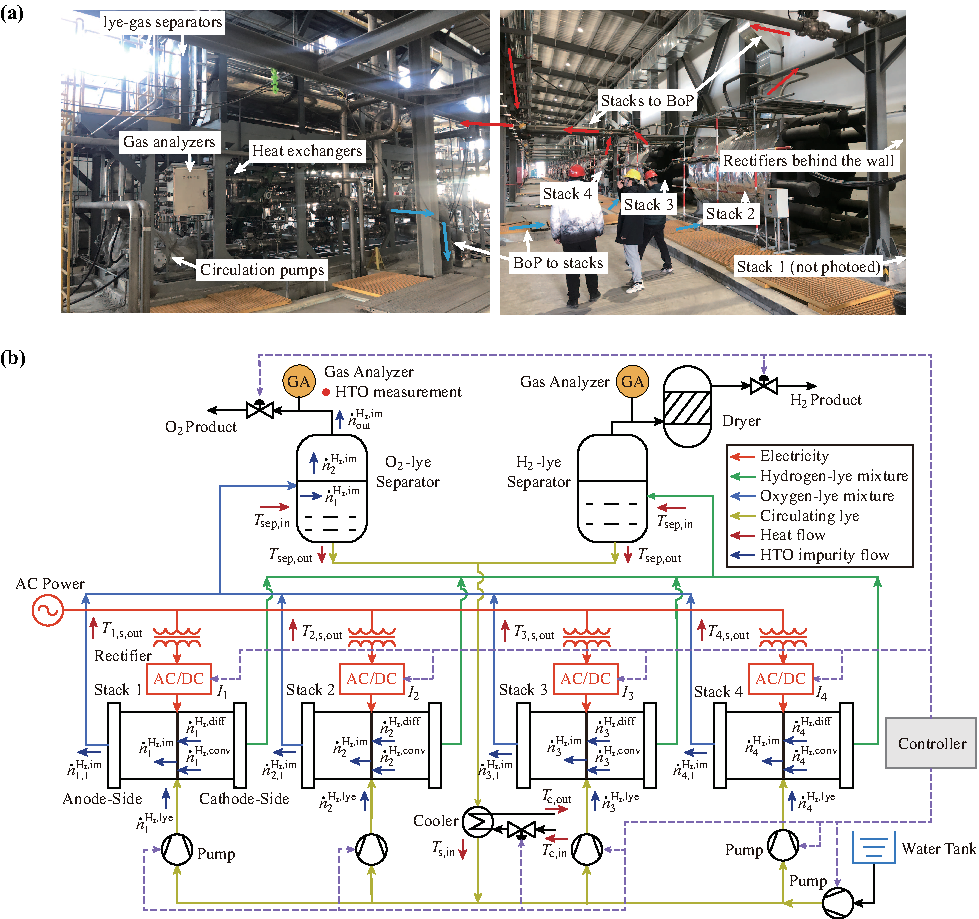
\includegraphics[scale=0.90]{sys}\vspace{-6pt}
	\caption{(a) Photo of 4-in-1 AWE systems in installation. (b) Schematic diagram of a typical 4-in-1 AWE system. }
	\label{fig:sys}
\end{figure}

On the electrical side, each stack is connected to a rectifier for dc power supply, allowing independent adjustment of load power. In some cases, a multi-winding transformer with phase-shift secondary windings replaces multiple transformers to reduce costs and minimize harmonic injections \cite{li2024two,zeng2024scheduling}. Note that some literature discusses multiple stacks sharing a single rectifier; however, due to challenges such as current equalization, insulation, and reduced flexibility, this configuration is not a common application.

The stacks are interconnected through the BoP, and their energy conversion efficiency, temperature, and HTO impurity accumulation under varying power inputs are directly influenced by controls on stack power, lye flow, and cooling. To capture the complex relation between control  and responses, this paper develops a state-space model of the $N$-in-1 system in Section \ref{sec:model} to support controller design.

\subsection{Assumptions}
\label{sec:assumptions}

%This study focuses on the efficiency, temperature, and HTO impurity accumulation behavior of $N$-in-1 systems during dynamic operations.
To simplify the model without loss of generality, the following assumptions are made:

\emph{a) Pressure Dynamics:} While pressure affects energy conversion efficiency \cite{ulleberg2003modeling}, and lowering the pressure can alleviate HTO accumulation %at low loads
to expand the load range \cite{qi2021pressure}, adjusting pressure may induce structural fatigue and reduce lifespan. Consequently, pressure adjustment is rarely employed in practice. In addition, pressure and liquid levels in separators are typically stabilized by independent PID controllers, which are effectively decoupled from efficiency, temperature, and HTO accumulation dynamics. Following related studies \cite{qi2021pressure,liang2024large,li2023exploration}, this work assumes the AWE system operates at a fixed pressure of 1.6 MPa. 
%, excluding the dynamic processes of pressure and level control.

\emph{b) Inter-Stack Stray Current:} Due to the pipeline between stacks being much longer compared to the channels in the stacks, stray currents are predominantly confined to the interior of the stacks \cite{dogan2024experimental}. %, with negligible stray currents between different stacks.
Thus, inter-stack stray currents are neglected. 
%, while the impacts of intra-stack stray currents on current efficiency, temperature, and impurity crossover are preserved.

\emph{c) Water Consumption and Replenishment:} The processes of water consumption and replenishment are much slower than the variations in current, temperature, and HTO impurity crossover, and these processes have minimal impact on control performance. Hence, they are neglected in this work.

\emph{d) Symmetry Between Stacks and BoP Components:} Many industrial AWE systems feature symmetric geometry design % and identical geometric parameters
for cathode- and anode-side flowsheets. %gas-liquid handling frameworks.
For simplicity, we assume thermal models are identical for both sides. %, leading to equal temperatures on the anode and cathode.
%Additionally, it is assumed that cooling water is supplied by a centralized utility system with a constant temperature.
Moreover, we assume the geometric parameters of the $N$ stacks are the same.


\section{State-Space Models of the $N$-in-1 AWE System}
\label{sec:model}

Compared to the 1-in-1 system, the dynamic behavior of the $N$-in-1 system is more complex due to the coupling of heat and mass flows between stacks. Based on the classical literature \cite{ulleberg2003modeling} and the authors' prior research on 1-in-1 systems %on thermal dynamics and impurity accumulation
\cite{qi2023thermal,qi2023design,qi2021pressure}, we establish a state-space model for the $N$-in-1 system.
Here, we will pay more attention to the unique aspects of the $N$-in-1 system while briefly introducing the components that also appear in 1-in-1 systems for completeness. The key variables are marked in Fig. \ref{fig:sys}(b). % for clarity.

\subsection{Electrochemical and Production Models}
\label{sec:production}

This process of converting electricity to hydrogen is described using the %electrochemical and 
production model. First, the cell voltage of each stack ($i=1,\ldots,N$) is modeled using the semi-empirical equations \cite{sanchez2018semi}:
\begin{align}
  U_i^{\rm{cell}} = U_i^{\rm{rev}} + \left(r_{i,1} +r_{i,2} T_{i,\text{s}} +r_{i,3} \rho \right) I_i
  + s_i \,{\rm{log}} \left[ \left( t_{i,1} +\frac{t_{i,2}}{T_{i,\text{s}}^2} +\frac{t_{i,3}} {T_{i,\text{s}}^2} \right) I_i +1\right], \label{eq:UItotal}
\end{align}
where $U_i^{{\rm{cell}}}$, $I_i$, and $T_{\text{s},i}$ are the cell voltage, current, and stack temperature; $U_i^{\rm{rev}}=1.23$ V is the reversible voltage; 
%determined by the Gibbs free energy \cite{onda2004prediction};
$\rho$ is the pressure; $r_{i,1}$, $r_{i,2}$, $r_{i,3}$, $s_{i}$, $t_{i,1}$, $t_{i,2}$ and $t_{i,3}$ are constant parameters.

Due to the existence of stray currents, not all current contributes to hydrogen production; some flows through the channels and dissipates. The current efficiency, known as \emph{Faraday efficiency}, is modeled by:
\begin{align}
  \eta_i^{\rm{cell}} = \frac{\left(0.1 I_i\right)^2}{f_{i,1} + \left( 0.1 I_i \right)^2} f_{i,2}, \label{eq:faraday}
\end{align}
where $f_{i,1}$ and $f_{i,2}$ are coefficients related to temperature and pressure.

%Considering each stack comprises $N^\text{cell}$ cells in series, the production rates of hydrogen and oxygen and power consumption for the $i$th stack are given by:
The hydrogen and oxygen production rates and power consumption of each stack are calculated as:
\begin{align}
  \dot{n}_{i}^{\text{H}_2,\text{prod}} &= { \eta_i^{\rm{cell}} N^{\rm{cell}} I_i}/{(2F)}, \label{eq:oxygenflow} \\
  \dot{n}_{i}^{\text{O}_2,\text{prod}} &= { \eta_i^{\rm{cell}} N^{\rm{cell}} I_i}/{(4F)}, \label{eq:hydrogenflow} \\
  P_i^{\rm{ele}} &= N^{\rm{cell}} U_i^{\rm{cell}} I_i,  \label{eq:power}
\end{align}
where $F=96,485$ C/mol is the Faraday's constant; $N^\text{cell}$ is the number of cells in a stack.

%The energy conversion efficiency depends nonlinearly on stack temperature, posing challenges for controller design (discussed in Section \ref{sec:simplification}). Additionally, parameters may vary over time due to degradation, necessitating online calibration \cite{qiu2023dynamic}.

Note that the energy conversion efficiency depends on stack temperature, showing a nonlinear coupling with the heat and mass transfer processes discussed in Section \ref{sec:thermal}.
This poses challenges for controller design. 
We later addressed them %through relaxation and approximation 
in Section \ref{sec:simplification}. Moreover, the parameters may vary due to degradation and can be calibrated via an online estimator developed in our prior study \cite{qiu2023dynamic}. The electrochemical model of individual stacks is the same as that of the 1-in-1 system and will not be elaborated.

%In operation, the electrochemical characteristics of the electrolyzer may change with time because of factors such as degradation, corrosion, and passivation. To accurately estimate the overvoltage, stress, and efficiency and provide a reference for thermal management, the above parameters need to be updated during online operation.

\subsection{Lye Circulation, Heat Transfer and HTO Impurity Accumulation Models}
\label{sec:process}

\subsubsection{Lye Circulation and Inter-Stack Distribution}
\label{sec:lye}

Typical lye circulation topologies for commercial $N$-in-1 systems are shown in Fig. \ref{fig:cir}. Some systems employ an independent pump for each stack, as shown in Fig. \ref{fig:cir}(a), allowing independent lye flow control. %In these cases, the flow rates $v_{i,\text{lye}}^{\text{ca/an}}$ for each stack can serve as independent control variables.
Other designs, such as Figs. \ref{fig:cir}(b) and \ref{fig:cir}(c), share pumps among multiple stacks. In these cases, lye flow distribution depends on the load of the stacks. % like electrolytic current.
%Without loss of generality, here we derive the lye flow distribution model based on the topology in Fig. \ref{fig:cir}(c).
Using Fig. \ref{fig:cir}(c) as an example, the lye flow distribution model is derived as follows.

\begin{figure}[t]
	\centering
	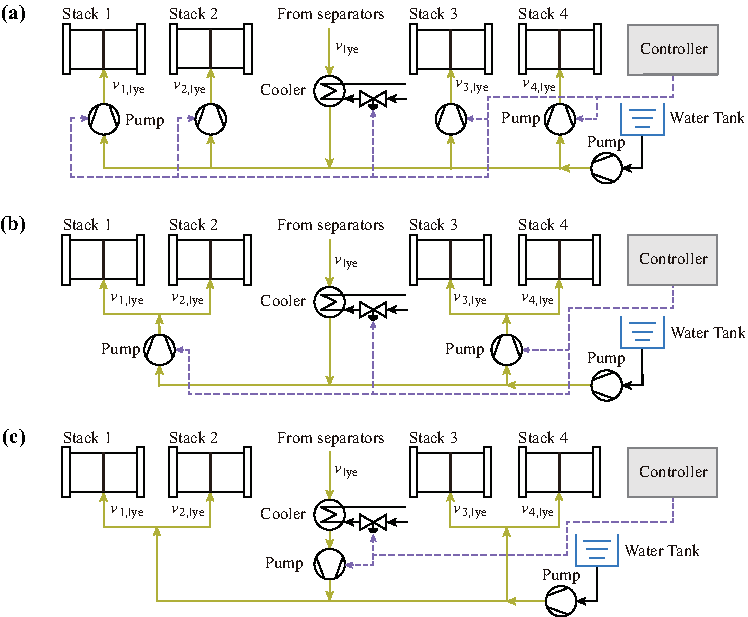
\includegraphics[scale=0.9]{cir}\vspace{-6pt}
	\caption{Topologies for inter-stack lye flow distribution. (a) 4 lye circulation pumps. (b) 2 lye circulation pumps. (c) 1 lye circulation pump.}
	\label{fig:cir}
\end{figure}

The flow rate of lye-gas mixture in each stack satisfies Poiseuille's law \cite{david2020dynamic}:
\begin{align}
  \Delta p_i = v_{i,\text{mix}}^{\text{ca/an}} R_i^{\text{ca/an}}, \label{eq:poiseuille}
\end{align}
\noindent
where $\Delta p_i$ is the pressure drop across the $i$th stack; $v_{i,\text{lye}}^{\text{ca/an}}$ is the flow rate of cathode/node-side lye-gas mixture; and $R_i^{\text{ca/an}}$ is the flow resistance.

As stacks are connected at both ends, as shown in Fig. \ref{fig:sys}(b), their pressure drops are identical. Therefore, the flow rates are inversely proportional to flow resistance:
\begin{align}
  \frac{v_{i,\text{mix}}^{\text{ca/an}}}{v_{j,\text{mix}}^{\text{ca/an}}} = \frac{R_i^{\text{ca/an}}}{R_j^{\text{ca/an}}}. \label{eq:lyeallocation}
\end{align}

Under laminar flow assumptions, $R_i^{\text{ca/an}}$ can be approximated as:
\begin{align}
  R_i^{\text{ca/an}} = \frac{128 \mu_{j,\text{mix}}^{\text{ca/an}} l }{\pi d^4}, \label{eq:flowresis}
\end{align}
where $l$ and $d$ are the equivalent length and diameter of the %anode/cathode-side 
flow paths; and $\mu_{j,\text{mix}}^{\text{ca/an}}$ is the dynamic viscosity of the lye-gas mixture, which can be approximated as a volume-weighted average of the dynamic viscosities of the lye $\mu_{\text{lye}}$ and the gas $\mu_{\text{H}_2/\text{O}_2}$ \cite{david2020dynamic}:
\begin{align}
  \mu_{i,\text{mix}}^{\text{ca/an}} = \frac{ V_{i,\text{gas}}^{\text{ca/an}} \mu_{\text{H}_2/\text{O}_2} + V_{i,\text{lye}}^{\text{ca/an}}   \mu_{\text{lye}}}{ V_{i,\text{gas}}^{\text{ca/an}} + V_{i,\text{lye}}^{\text{ca/an}}}
  = \alpha_{i}^{\text{ca/an}}  \mu_{\text{H}_2/\text{O}_2} +  \left( 1- \alpha_{i}^{\text{ca/an}}  \right) \mu_{\text{lye}},  \label{eq:viscos}
\end{align}
\noindent
where $V_{i,\text{lye}}^{\text{ca/an}}$ and $V_{i,\text{gas}}^{\text{ca/an}}$ are the volumes of the lye and gas in the $i$th stack; $\alpha_{i}^{\text{ca/an}}$ represents the volumetric gas ratio, calculated as:
\begin{align}
  \alpha_{i}^{\text{ca/an}} =  \frac{V_{i,\text{gas}}^{\text{ca/an}}}{V_{i,\text{gas}}^{\text{ca/an}} + V_{i,\text{lye}}^{\text{ca/an}}} =  \frac{\dot{n}_{i}^{\text{H}_2/\text{O}_2,\text{prod}} R T_{\text{s},i} }{\rho v_{i,\text{mix}}^{\text{ca/an}}},
\end{align}
\noindent
where $R$ is the gas constant.

The flow rates of gas and lye $v_{i,\text{gas}}^{\text{ca/an}}$ and $v_{i,\text{lye}}^{\text{ca/an}}$ can be then extracted as: % from the flow rates of the mixture:
\begin{subnumcases}{\label{eq:vlye}}
  v_{i,\text{gas}}^{\text{ca/an}}  = \alpha_{i}^{\text{ca/an}} v_{i,\text{mix}}^{\text{ca/an}}, \label{eq:vlyegas} \\
  v_{i,\text{lye}}^{\text{ca/an}}  =  \left( 1- \alpha_{i}^{\text{ca/an}} \right) v_{i,\text{mix}}^{\text{ca/an}}, \label{eq:vlyelye}
\end{subnumcases}
\noindent
which are later used for the thermal and HTO impurity models in Sections \ref{sec:thermal} and \ref{sec:hto}.

From the above discussion, we know that the gas ratio is related to gas production. %, and thus to the electrolytic power. 
Different electrolytic power leads to varying gas ratios, affecting flow resistances and consequently the inter-stack lye flow distribution. Compared with the 4-pump topology in Fig. \ref{fig:cir}(a), the 1-pump topology in Fig. \ref{fig:cir}(c) has less flexibility in regulating lye flow. Nevertheless, with appropriate control, the system's performance %in load tracking, temperature stabilizing, and optimizing energy conversion efficiency 
will not be adversely affected, as detailed in Section \ref{sec:comparetopo}.

\begin{remark}
  \label{remark:1}
  Considering that the viscosity of gases (around 0.9$\times$10$^{-\text{5}}$ Pa$\cdot$s for hydrogen and 2.2$\times$10$^{-\text{5}}$ Pa$\cdot$s for oxygen) is orders of magnitude lower than that of lye (around 2.3$\times$10$^{-\text{3}}$ Pa$\cdot$s), i.e., $\mu_{\text{H}_2/\text{O}_2} \ll \mu_{\text{lye}}$, the former can be neglected in (\ref{eq:viscos}), yielding $\mu_{i,\text{mix}}^{\text{ca/an}} \approx \big( 1-\alpha_i^{\text{ca/an}}\big) \mu_{\text{lye}} $.
  Further, by comparing (\ref{eq:vlyegas}) and (\ref{eq:vlyelye}), it follows that for different $i$ and $j$, we have $v_{i,\text{lye}}^{\text{ca/an}} \approx v_{j,\text{lye}}^{\text{ca/an}}$, meaning that even if the operating points of the stacks differ, the liquid-phase flow can be considered to distribute evenly.
  Moreover, the lye flow rates on the cathode and anode sides can be assumed equal, i.e., $v_{i,\text{lye}}^{\text{ca}} \approx v_{i,\text{lye}}^{\text{an}}$. We further denote $v_{i,\text{lye}} = v_{i,\text{lye}}^{\text{ca}} + v_{i,\text{lye}}^{\text{an}}$. %These reduce nonlinearity and simplify the design of the controller in Section \ref{sec:control}.
\end{remark}

\subsubsection{Heat Transfer}
\label{sec:thermal}

Temperature affects the efficiency, safety, and flexibility of the AWE systems. As shown in Section \ref{sec:production}, low temperature increases overvoltage, reducing energy conversion efficiency, while excessively high temperature imposes excessive thermal stress, shortening the lifespan of electrodes, diaphragm, and sealing materials. For the 1-in-1 AWE system, our previous studies \cite{qi2023thermal}
proposed a 3rd-order state-space model to capture the heat transfer behaviors among the stack, separators, and heat exchanger. In this work, we further extend this model to $N$-in-1 AWE systems.

In an $N$-in-1 system, the temperature of each stack and its internal lye flow is jointly determined by electrolytic heat, lye-gas flow, and heat dissipation to the environment, modeled as:
\begin{align}
  C_{i,\text{s}} \dfrac{{\text{d}}T_{i,\text{s,out}}}{\text{d}t} = Q_{i,\text{ele}} - Q_{i,\text{s,diss}} - c_{\text{lye}} v_{i,\text{lye}} \rho_{\rm{lye}} \left( T_{i,\text{s,out}} - T_{i,\text{s,in}} \right), \label{eq:heatstack}
\end{align}
where $C_{i,\text{s}}$ denotes the total heat capacity of the stack and the lye inside it, i.e., $C_{i,\text{s}} = C_{i,\text{struc,s}} + C_{i,\text{lye,s}}$, with $C_{i,\text{lye,s}} = V_{i,\text{s,lye}} \rho_\text{lye} c_\text{lye}$; $V_{i,\text{s,lye}}$ is the volume of the lye in the stack; $\rho_\text{lye} = 1,250\ \text{kg}/\text{m}^{3}$ and $c_\text{lye} = 3,300\ \text{J}/(\text{kg}\cdot{K})$  are the density and specific heat capacity of the lye; $T_{i,\text{s,in}}$/$T_{i,\text{s,out}}$ denotes the inlet/outlet lye temperature the $i$th stack; %(for convenience, referred to hereafter as \emph{pre-stack} and \emph{post-stack} temperatures, respectively).  ;
$Q_{i,\text{ele}}$ denotes heating flow; $Q_{i,\text{diss,s}}$ denotes heat dissipation to the environment. %The heat carried away by gases is neglected here.

Note that, as indicated in Fig. \ref{fig:sys}(b), the inlet temperature of the stacks %in an $N$-in-1 system 
is the same, while the outlet temperature varies due to differences in the temperature and load among stacks.

The heating flow $Q_{i,\text{ele}}$ comprises the heat released by the electrolytic reaction and the ohmic heat from the stray current, as:
\begin{align}
  Q_{i,\text{ele}} = \eta_i^{\text{cell}} N^{\text{cell}} I_i \left( U_i^{\text{cell}} - U^{\text{th}} \right) + \left( 1 - \eta_i^{\text{cell}} \right) N^{\text{cell}} I_i U_i^{\text{cell}}, \label{eq:heatele}
\end{align}
where $U^\text{th}=1.48$ V is the thermoneutral voltage. %The left term represents the reaction heat of water electrolysis, and the right term represents the ohmic heat from the stray current.

Heat dissipation $Q_{i,\text{s,diss}}$ from the $i$th stack to the environment includes convection and radiation, denoted as $Q_{i,\text{s,conv}}$ and $Q_{i,\text{s,rad}}$, which follow:
\begin{align}
  Q_{i,\text{s,diss}} = Q_{i,\text{s,conv}} + Q_{i,\text{s,diss}} = h_\text{s} A_{\text{s,diss}} ( T_{i,\text{s,out}} - T_\text{am}) + \sigma A_{\text{s,diss}} \epsilon_\text{s} ( T^4_{i,\text{s,out}} - T^4_\text{am} ), \label{eq:heatdiss}
\end{align}
where %$Q_{i,\text{s,conv}}$ and $Q_{i,\text{s,diss}}$ denote the heat loss due to natural convection and radiation, respectively;
$A_{\text{s,diss}}$ is the %equivalent
 heat dissipation area; %of the stack;
$T_\text{am}$ is the ambient temperature; $\sigma$ is the Stefan-Boltzmann constant; $\epsilon_\text{s}$ denotes the emissivity of the stack; and $h_\text{s}$ is the natural convection %heat transfer 
coefficient, %. Considering the stack is a cylinder with , the emissivity $\epsilon_\text{s}$ can be calculated by %based on its geometry and the temperature difference between it and the environment 
following \cite{dieguez2008thermal}:
\begin{align}
  h_\text{s} = 2.51 \times 0.52 \left[ \left( {T_{i,\text{s,out}} - T_{\text{am}}}  \right) / {\phi_{s}} \right]^{0.25}, \label{eq:disscoef}
\end{align}
where $\phi_{s}$ represents the diameter of the stack.

As indicated in Fig. \ref{fig:sys}, the lye exiting the $N$ stacks is mixed before entering the separators. Assuming no heat loss in pipes, the separator inlet temperature $T_{\text{sep,in}}$ is the weighted average of the outlet lye temperatures of the $N$ stacks: %based on the lye flow rates,
\begin{align}
  T_{\text{sep,in}} = \dfrac{ \sum_{i=1}^N v_{i,\text{lye}} T_{i,\text{s,out}} } {v_{\text{tot,lye}}},
\end{align}
where %$T_{\text{sep,in}}$ is the temperature of the lye entering the separators;
$v_{\text{tot,lye}} = \sum_{i=1}^N v_{i,\text{lye}}$ denotes total lye flow.

For the separators, assuming the heat carried by gaseous hydrogen/oxygen is negligible, the temperature is determined by % the heat brought in by the lye from the stacks, carried away by the outgoing lye and dissipation, as follows:
\begin{align}
  C_{\text{sep}} \dfrac{{\text{d}}T_{\text{sep,out}}}{\text{d}t} = \frac{1}{2} c_{\text{lye}} v_{\text{tot,lye}} \rho_{\rm{lye}} \left( T_{\text{sep,in}} - T_{\text{sep,out}} \right) - Q_{\text{sep,conv}} - Q_{\text{sep,rad}}  , \label{heatseparator}
\end{align}
where $C_{\text{sep}}$ is the heat capacity of the separator and lye inside it; $T_{i,\text{sep,out}}$ is the separator outlet temperature; $Q_{\text{sep,conv}}$ and $Q_{\text{sep,rad}}$ are the convective and radiative dissipation, calculated similarly to (\ref{eq:heatdiss})--(\ref{eq:disscoef}). % and thus omitted here.

The lye left the cathode and anode-side separators is mixed and cooled before being circulated to the stack. Assuming the heat exchanger is a commonly used counterflow type, we have %its temperature behavior is modeled as:
\begin{align}
  C_{\text{he}} \dfrac{{\text{d}}T_{\text{s,in}}}{\text{d}t} = c_{\text{lye}} v_{\text{tot,lye}} \rho_{\rm{lye}} \left( T_{\text{sep,out}} - T_{\text{s,in}} \right) - k A_\text{c} \Delta T  , \label{eq:heatexchange}
\end{align}
where $C_{\text{he}}$ is the total heat capacity of the heat exchanger and lye it contains; % as $C_{\text{he}}= C_{\text{he,liq}} + C_{\text{he,struc}}$;
$A_\text{c}$ represents heat exchange area; $k$ is the heat transfer coefficient; and $\Delta T$  is the logarithmic temperature difference, as:
\begin{align}
  \Delta T = \frac{ \left( T_{\text{s,in}} - T_{\text{c,out}} \right) - \left( T_{\text{sep,out}} - T_{\text{c,in}} \right) }{\log \left[ \left( T_{\text{s,in}} - T_{\text{c,out}} \right) / \left( T_{\text{sep,out}} - T_{\text{c,in}} \right) \right]},
\end{align}
where $T_{\text{c,in}}$ denotes the inlet cooling water temperature, which is regulated by a chiller and we assume it to be constant; $T_{\text{c,out}}$ denotes the outlet temperature of cooling water, determined as follows:
\begin{align}
  C_{\text{c}} \dfrac{{\text{d}}T_{\text{c,out}}}{\text{d}t} = c_{\text{c}} v_{\text{c}} \rho_{\text{c}} \left( T_{\text{c,in}} - T_{\text{c,out}} \right) + k A_\text{c} \Delta T  , \label{eq:heatcooling}
\end{align}
where $C_{\text{c}}$ denotes the total heat capacity of the cooling coil and the cooling water it contains; %i.e., $C_{\text{c}} = C_{\text{c,liq}} + C_{\text{c,struc}}$, with the heat capacity of the cooling water satisfying $C_{\text{c,liq}} = V_{\text{c}} c_{\text{c}} \rho_{\text{c}}$. Here, $V_{\text{c}} $ is the volume of cooling water in the coil,
$c_{\text{c}}=4,100$ J/(kg$\cdot$K) and $\rho_{\text{c}} = 1,000$ kg/m$^3$ are the specific heat capacity and density of the cooling water, respectively; and $v_{\text{c}}$ represents the cooling water flow rate, which is regulated by a valve.

For an $N$-in-1 system, the heat transfer model (\ref{eq:heatstack})--(\ref{eq:heatcooling}) has an order of $N+3$. %, compared with the $3$rd-order for a 1-in-1 system in \cite{qi2023thermal}.
%Based on this model, the temperature behavior of the stacks, separators, and heat exchanger can be evaluated, which is jointly determined by the control of electrolytic load, lye circulation, and cooling water flow. 
This model links temperature dynamics with control of electrolytic load, lye flow, and cooling water.
The temperatures also appear in the electrochemical model in Section \ref{sec:production} and the HTO impurity accumulation model in Section \ref{sec:hto}, %as variable parameters,
showing coupling relations, which is addressed in the controller design in Section \ref{sec:control}. % forming a basis for optimizing the operational temperature control of the electrolyzer.


\subsubsection{HTO Impurity Accumulation}
\label{sec:hto}

Gas crossover between the anode and cathode sides occurs due to the non-compactness of the diaphragm and the mixing of lye returned from the hydrogen-side and oxygen-side separators. %Hydrogen, being smaller and produced at twice the rate of oxygen, crosses to the anode side more rapidly. 
Once the HTO impurity concentration reaches half the flammability limit (2 vol\%), the safety system shuts down the electrolyzer to prevent explosions \cite{sanchez2018semi}. Since HTO impurity accumulation impacts the lower load limit, it must be accounted for in controller design.
%Due to the non-compactness of the diaphragm and the mixture of lye returned from the hydrogen- and oxygen-size separators, gas crossover occurs between the anode and cathode sides. Specifically, hydrogen, being a smaller molecular and produced at twice the rate of oxygen, crosses to the anode side more quickly. Once the concentration of HTO impurity reaches half of the flammability limit (typically 2 vol\%), the safety system shuts down the electrolyzer to prevent explosions \cite{sanchez2018semi}.
%Because the accumulation of HTO impurity is a dynamic process that affects the lower load limit, the controller design must account for it.
Here, we extend the 3rd-order model for 1-in-1 systems proposed in our previous work \cite{qi2021pressure} to the $N$-in-1 system.
%The relationship between the HTO impurity accumulation and operating conditions such as the load allocation among the multiple stacks, lye circulation, and temperature are established in detail.

In each stack of the $N$-in-1 system, the HTO impurity crossovers from the cathode-side half-cell to the anode-side half-cell via lye circulation \cite{david2020dynamic}, diffusion \cite{trinke2018hydrogen}, and convection \cite{trinke2018hydrogen}:
\begin{align}
  \dot{n}^{\text{H}_2,\text{im}}_i = \dot{n}^{\text{H}_2,\text{lye}}_i +  \dot{n}^{\text{H}_2,\text{diff}}_i +  \dot{n}^{\text{H}_2,\text{conv}}_i  , \label{eq:nim}
\end{align}
\noindent
%where $\dot{n}^{\text{H}_2,\text{lye}}_i$, $\dot{n}^{\text{H}_2,\text{diff}}_i$, and $\dot{n}^{\text{H}_2,\text{conv}}_i$ are
where $n^{\rm{H_2}}_{\rm{lye}}$, $n^{\rm{H_2}}_{\rm{lye}}$, and $n^{\rm{H_2}}_{\rm{conv}}$ are the molar flows of HTO impurity brought in by lye circulation, diffusion, and convection, respectively. %The corresponding molar flows are given as:

As shown in Fig. \ref{fig:sys}, the circulating lye contains dissolved hydrogen due to the mixing of the return flows from hydrogen-side and oxygen-side separators. The corresponding molar flow of HTO impurity, $\dot{n}^{\text{H}_2,\text{lye}}_i$, depends on the distribution of lye flow across the $N$ stacks (see Section \ref{sec:lye}), following \cite{david2020dynamic}:
\begin{align}
  \dot{n}^{\text{H}_2,\text{lye}}_i = { S^{\rm{H_2}} \rho v_{i,\text{lye}}}/{4},\label{eq:nlye}
\end{align}
where $S^{\rm{H_2}}$ is the solubility of hydrogen in the lye.

The crossover molar flows of HTO impurities due to diffusion and convection,  $\dot{n}^{\text{H}_2,\text{diff}}_i$ and $\dot{n}^{\text{H}_2,\text{conv}}_i$, are determined by Fick's law and Darcy's law \cite{trinke2018hydrogen}, respectively, as:
\begin{subnumcases}{\label{eq:hto}} 
  \dot{n}^{\text{H}_2,\text{diff}}_i  = A^{\text{cell}} N^{\text{cell}} \frac{D^{\text{H}_2}_{\text{eff}} \Delta c^{\rm{H_2}}}{\delta} \approx A^{\text{cell}} N^{\text{cell}} \frac{D^{\text{H}_2}_{\text{eff}} S^{\text{H}_2} \rho}{\delta},\label{eq:ndiff} \\
  \dot{n}^{\text{H}_2,\text{conv}}_i  = A^{\text{cell}} N^{\text{cell}} \frac{K^{\text{H}_2}_{\text{eff}}}{\mu_{i,\text{lye}}} S^{\text{H}_2} \rho \frac{\Delta \rho}{\delta},\label{eq:nconv}
\end{subnumcases}
where %$n^{\rm{H_2}}_{\rm{im}}$ is the hydrogen impurity flow rate into the anode half-cell; $n^{\rm{H_2}}_{\rm{lye}}$, $n^{\rm{H_2}}_{\rm{lye}}$, and $n^{\rm{H_2}}_{\rm{conv}}$ represent the molar flows caused by lye circulation, diffusion, and convection;
$D^{\rm{H_2}}_{\rm{eff}}$ is the diffusion coefficient; % of hydrogen in the lye; 
$\Delta c^{\rm{H_2}}$ denotes the differential concentration of hydrogen between the cathode and anode sides; $\delta$ is the thickness of the diaphragm; $K^{\text{H}_2}_{\text{eff}}$ is the permeability of the hydrogen through the diaphragm; $\Delta \rho$ denote the pressure difference between two sides, usually caused by fluctuations in pressure and liquid levels. % control.

The HTO impurity is transported and accumulates throughout the system in three stages, including the anode half-cell, the liquid phase of the separator, and the gas phase of the separator, as shown in Fig. \ref{fig:sys}. 
Based on molar volume conservation, we establish a state-space model for HTO accumulation in the $N$-in-1 system, similar to our prior work \cite{qi2021pressure}, as:
%, we establish a state-space model for HTO accumulation in the $N$-in-1 system based on molar volume conservation, as follows:
\begin{subnumcases}{\label{eq:Nbalance}}
  \dfrac{ \text{d} n^{\text{H}_2,\text{an}}_{i}} {\text{d}t} = \dot{n}^{\text{H}_2,\text{im}}_{i} - \dot{n}^{\text{H}_2,\text{im}}_{i,1}, \ i=1, \ldots, N, \\
  \dfrac{\text{d} n^{\text{H}_2,\text{sep}}_{\text{liq}}}{\text{d}t} = \sum\nolimits_{i=1}^{N} \dot{n}^{\text{H}_2,\text{im}}_{i,1} - \dot{n}^{\text{H}_2,\text{im}}_2,  \\
  \dfrac{\text{d} n^{\text{H}_2,\text{sep}}_{\text{gas}}}{\text{d}t} = \dot{n}^{\text{H}_2,\text{im}}_{2} - \dot{n}^{\text{H}_2,\text{im}}_{\text{out}},
\end{subnumcases}
where $n^{\text{H}_2,\text{an}}_{i}$, $ n^{\text{H}_2,\text{sep}}_{\text{liq}}$, and $\text{d} n^{\text{H}_2,\text{gas}}_{\text{gas}}$ represent the molar quantities of HTO impurity in the anode half-cell of the $i$th stack, and the liquid and gas phases of the separator, respectively; $ \dot{n}^{\text{H}_2,\text{im}}_{i,1}$, $\dot{n}^{\text{H}_2,\text{im}}_2$, and $\dot{n}^{\text{H}_2,\text{im}}_{\text{out}}$ are the molar flows of HTO impurity, %, as illustrated by the blue arrows in Fig. \ref{fig:sys},
which satisfies:
\begin{subnumcases}{\label{eq:nbalance}}
  \dot{n}^{\text{H}_2}_{i,1} = \frac{n^{\text{H}_2,\text{an}} v_{i,\text{lye}} }{2 V^{\text{an}}_{\text{lye}}}, \ i=1,\ldots,N,\\
  \dot{n}^{\text{H}_2}_2 =\frac{N^{\rm{H_2,sep}}_{\rm{liq}}}{\tau_{\rm{sep}}}, \\
  \dot{n}^{\text{H}_2}_{\rm{out}}=  \frac{R T_{\text{sep,out}} N^{\text{H}_2,\text{sep}}_{\text{gas}} \sum\nolimits_{i=1}^{N} n^{\text{O}_2,\text{prod}}_i} {\rho V_{\rm{sep,gas}}}, \label{eq:nbalance3}
\end{subnumcases}
where $V^{\rm{lye}}_{\rm{an}}$ is the volume of lye in the anode-side half-cell; $\tau_{\rm{sep}}$ is the separation time constant; $V_{\rm{sep,gas}}$ is the gas-phase volume of the separator.

The HTO impurity concentration in the gas phase of the oxygen-side separator, which is measured and taken as the safety metric \cite{david2020dynamic,trinke2018hydrogen,qi2021pressure}, follows:
\begin{align}
  \text{HTO} = \frac{n^{\text{H}_2,\text{sep}}_{\text{gas}} R T_{\text{sep,out}}} {\rho V_{\text{sep,gas}}}. \label{eq:defhto}
\end{align}
%where $n^{\text{H}_2,\text{im,sep}}$ is the molar quantity of hydrogen impurities at the gas phase of the separator;

Compared to the 1-in-1 system model in \cite{qi2021pressure}, the model order of the $N$-in-1 system increases to $N$+2. The accumulation process depends not only on the overall power but also on inter-stack load allocation and lye flow control, significantly increasing the complexity. 
The HTO impurity accumulation process is also integrated into the controller to accommodate the varying energy input; %through coordinated control of the electrolytic load and lye flow; 
see Section \ref{sec:control} for details.

\subsection{Model Summary}
\label{sec:modelsummary}

Summarizing the %electrochemical and production models, electrolyte distribution between electrolyzers, HTO impurity accumulation, and temperature
submodels established in Sections \ref{sec:production} and \ref{sec:process}, %\ref{sec:lye}, \ref{sec:thermal}, and \ref{sec:hto}, 
Table \ref{tab:model} presents an overview of the state-space model for the $N$-in-1 AWE system. Note that the electrochemical and inter-stack lye distribution submodels are formulated by algebraic equations. Their state spaces are zero in dimension. Consequently, the complete state-space model has an order of $2N+5$.

\begin{table}[tb]\scriptsize\centering
  \renewcommand{\arraystretch}{1.35}
  \caption{Summary of the proposed state-space model of the $N$-in-1 AWE system}\vspace{6pt}
  \label{tab:model}
  \begin{tabular}{ ccccc }\hline\hline
  Submodel              & \tabincell{c}{Electrochemical\\ and production}   & \tabincell{c}{Lye flow\\distribution} & \tabincell{c}{Heat transfer}                & \tabincell{c}{HTO impurity accumulation} \\ \hline
  State variables       & /                                                 & /                                                 & $T_{\text{s,in}}$, $\big\{ T_{i,\text{s,out}} \big\}_{i=1}^N$, $T_{\text{sep,out}}$, $T_{\text{c,out}}$                                              & $\big\{ n_i^{\text{H}_2,\text{an}} \big\}_{i=1}^N$,  $ n_{\text{liq}}^{\text{H}_2,\text{sep}}$,  $ n_{\text{gas}}^{\text{H}_2,\text{sep}} $                                         \\
  Order of model        & $0$                                               & $0$                                               & $N+2$                                         & $N+3$ \\
  Formulation           & (\ref{eq:UItotal})--(\ref{eq:power})              & (\ref{eq:poiseuille})--(\ref{eq:vlye})            & (\ref{eq:heatstack})--(\ref{eq:heatcooling})  & (\ref{eq:nim})--(\ref{eq:defhto})\\
  Control variables     &  \multicolumn{4}{c}{ Electrolytic currents $\big\{ I_i \big\}_{i=1}^N$, lye flow rates $\big\{ v_{i,\text{lye}} \big\}_{i=1}^N$, and cooling water flow rates $v_\text{c}$}        \\
  \hline\hline
  \end{tabular}
\end{table}

\begin{figure}[t]
	\centering
	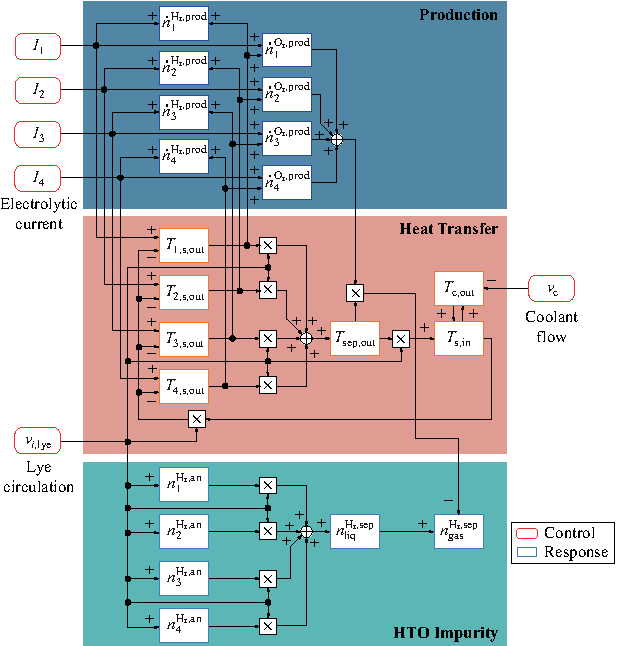
\includegraphics[scale=0.90]{state}\vspace{-6pt}
	\caption{Interrelationships between state variables, control, and responses in the $N$-in-1 AWE system with the 1-pump topology in Fig. \ref{fig:cir}(c).}
	\label{fig:state}
\end{figure}

For easy understanding, Fig. \ref{fig:state} provides an illustration of the interrelationships among control and responses.
We can observe that processes of hydrogen production, thermal dynamics, and HTO impurity accumulation are mutually coupled; %Some control actions even oppositely affect a same variable.
%For example, increasing the electrolytic current not only raises hydrogen production but also elevates the stack temperature and accelerates the discharge of HTO impurities, thereby reducing the HTO concentration. On the other hand, increasing the lye flow rate lowers the temperatures in the stacks and separators, but increases HTO accumulation; 
see examples in Section \ref{sec:openloop}.
Furthermore, compared to the 1-in-1 system, the $N$-in-1 system features greater control freedom, as the current and lye flow distribution among the stacks can be adjusted. This increases the dimensionality of the control action space, making it more challenging to find the optimal control.

For the convenience, % of controller modeling, 
we summarize the state and control variables in vector forms:
\begin{gather}
  \bm{x} \triangleq \big[ T_{\text{s,in}}, T_{1,\text{s,out}}, \ldots, T_{N,\text{s,out}}, T_{\text{sep,out}}, T_{\text{c,out}}, n_1^{\text{H}_2,\text{an}}, \ldots, n_N^{\text{H}_2,\text{an}}, n_{\text{liq}}^{\text{H}_2,\text{sep}}  , n_{\text{gas}}^{\text{H}_2,\text{sep}} \big]^{\text{T}}, \label{eq:state} \\
  \bm{u}  \triangleq \big[  I_1, \ldots, I_N, v_{1,\text{lye}}, \ldots, v_{N,\text{lye}}, v_\text{c} \big]^{\text{T}}, \label{eq:control}
\end{gather}
\noindent
and compactly express the state equations as:
\begin{align}
  {\text{d}\bm{x}}/{\text{d}t} = \bm{h}(\bm{x}, \bm{u}). \label{eq:equstate}
\end{align}

\section{Controller Design}
\label{sec:control}

\subsection{Overview of Control}

Section \ref{sec:modelsummary} shows that the $N$-in-1 AWE system is a complex multi-input multi-output (MIMO) system, making it challenging to ensure both safety and efficiency under fluctuating power inputs. %Existing studies, %on AWE system control,
%as reviewed in Section \ref{sec:review}, do not consider the topology of sharing separators or the process of HTO impurity accumulation, and they often rely on static optimization or rule-based control laws \cite{zheng2022optimal,liang2024large,li2023exploration}  which cannot ensure optimality during dynamic operation. Moreover, 
Due to the MIMO characteristics and strong nonlinearity, %of the AWE system, 
PID \cite{qi2023design,qi2021pressure} or model predictive control (MPC) based on linearization are not suitable \cite{baldea2014integrated}. To address these challenges with full consideration of the nonlinear MIMO characteristics, this paper developed a nonlinear model predictive controller (NMPC) %as an advanced process controller (APC)
for the $N$-in-1 AWE system. %, aiming to improve adaptability to fluctuating power sources.

As in the classical MPC, we consider a control horizon $N^\text{h}$ and a step length $\Delta t$ for time-domain discretization. Given the large time constants of the temperature and HTO accumulation processes, typically on the order of tens of minutes, a longer horizon is required, and a large step length is desired to reduce the size of the optimization problem. %of the optimization model.
Therefore, we use the trapezoidal format to discretize (\ref{eq:equstate}) in the time domain to ensure accuracy and numerical stability:
\begin{align}
  \frac{\bm{x}(k+1) - \bm{x}(k) }{\Delta t} = \frac{\bm{h}\big( \bm{x}(k+1), \bm{u}(k+1) \big) + \bm{h}\big( \bm{x}(k), \bm{u}(k) \big)}{2}, \ k = 0, \ldots, N^{\text{h}}-1, \label{eq:diststate}
\end{align}

Additionally, the control objectives and constraints are established as follows.

\subsection{Control Objective}
\label{sec:obj}

The primary control objective is to maximize hydrogen production % and energy conversion efficiency %and reduce the levelized cost of hydrogen (LCOH)
while tracking the fluctuating energy input. Meanwhile, stack temperature should be stabilized to reduce thermal stress, and repeated adjustments of lye/cooling water flow should be minimized to alleviate fatigue. To achieve these goals, the overall objective function of the controller is set as:
\begin{align}
  f\big( \bm{x}(1), \ldots, \bm{x}(N^\text{h}), & \bm{u}(0), \bm{u}(1), \ldots, \bm{u}(N^\text{h}) \big) = - \lambda^{\text{prod}} \Delta t \sum\nolimits_{k=0}^{N^\text{h}} \sum\nolimits_{i=1}^{N} \dot{n}_{i}^{\text{H}_2,\text{prod}}  \nonumber \\
  + & \lambda^{\text{track}} \sum\nolimits_{k=0}^{N^\text{h}} \Big( P_{\text{tot}}^{\text{ref}}(k) - \sum\nolimits_{i=1}^{N} P_{i}^{\text{ele}}(k) \Big)^2  \nonumber \\
  + & \lambda^{\text{temp}} \sum\nolimits_{k=0}^{N^\text{h}} \sum\nolimits_{i=1}^{N} \Big( T_{i,\text{s,out}}(k) -  T_{\text{s,out}}^{\text{ref}} \Big)^2  \nonumber \\
  + & \lambda^{\text{I}} \sum\nolimits_{k=0}^{N^\text{h}-1} \sum\nolimits_{i=1}^{N} \Big( I_{i}(k+1) -  I_{i}(k) \Big)^2  \nonumber \\
  + & \lambda^{\text{lye}} \sum\nolimits_{k=0}^{N^\text{h}} \sum\nolimits_{i=1}^{N} \Big( v_{i,\text{lye}}(k) -  v_{i,\text{lye}}^{\text{0}} \Big)^2  \nonumber \\
  + & \lambda^{\text{c}} \sum\nolimits_{k=0}^{N^\text{h}}  \Big( v_{\text{c}}(k) -  v_{\text{c}}^{0} \Big)^2,
   \label{eq:obj}
\end{align}
\noindent
where $P_{\text{tot}}^{\text{ref}}$ is the reference for total power consumption; $T_{\text{s,out}}^{\text{ref}}$ is the temperature reference for the $i$th stack; $\lambda^{\text{prod}}$, $\lambda^{\text{track}}$, $\lambda^{\text{temp}}$, $\lambda^{\text{I}}$, $\lambda^{\text{lye}}$, and $\lambda^{\text{c}}$  are weights for hydrogen production, load tracking, temperature stabilization, and electrolytic current, lye circulation and cooling water flow adjustments.

For power tracking, i.e., the second row in (\ref{eq:obj}), three application scenarios are considered:
\begin{enumerate}
  \item{Tracking renewable energy.} Forecasts of wind and solar power are used as the power reference $P_{\text{tot}}^{\text{ref}}(k)$, and the forecast error is alleviated through the rolling implementation of NMPC.
      Techniques such as robust control \cite{li2024two} %or stochastic control \cite{qiu2020stochastic}
      can be used to improve performance under uncertainty.

  \item{Participating in peak-shaving for the power grid: Power references are issued by grid operators in advance, which is a deterministic time series. }

  \item{ Tracking automatic generation control (AGC) signals}: Given the high uncertainty, non-Gaussian characteristics, and temporal correlations of AGC signals, the dynamic response of the AWE system should be treated as a stochastic process and addressed with stochastic MPC (SMPC), as demonstrated in prior studies \cite{qiu2021continuous,qiu2020stochastic}. Since this paper focuses on the AWE system, deterministic power references are considered, leaving SMPC for future research.
\end{enumerate}


\subsection{Constraints}
\label{eq:constraints}

At each time step $(k = 1,\ldots, N^\text{h})$ and for each stack $(i=1,\ldots,N)$, the following constraints must be satisfied to ensure operational feasibility and safety.

\subsubsection{DC Power and Cell Voltage Constraints}

%From the electrochemical model (\ref{eq:UItotal}), we can see that when stack temperature is higher, the feasible load range is higher.
 %and the flexibility is better \cite{qiu2024flexibility}. %In addition, the load upper limit constraint during the cold startup process can also be characterized by the cell voltage constraint \cite{qiu2023extended}.
The rectifier that provides DC power has current and power limits, 
% due to device current resistance, heat dissipation, and other limitations,
expressed as:
\begin{gather}
  0 \le I_i^\text{cell}(k) \le \overline{I}, \ \text{and} \  %\label{eq:limitdccurrent} \\
  0 \le P^\text{ele}_i(k) \le \overline{P}^\text{ele}, \label{eq:limitdcpower}
\end{gather}
\noindent
where $\overline{I}$ and $\overline{P}^\text{ele}_i$ are the current and power limits that the rectifier can provide, which is usually $1.2$ to $1.4$ times the rated power of the stack. % to meet a certain overload capacity. (Overload control is not considered in this article).

Moreover, to avoid excessive stress on electrodes and catalysts, the cell voltage is limited:
\begin{align}
  U_i^\text{cell}(k) \le \overline{U}^\text{cell}, \label{eq:limitcellvolt}
\end{align}
where $\overline{U}^\text{cell}$ is typically set at $2.1$ to $2.3$ V. 

Note that some studies \cite{rizwan2021design,chen2024enhancing,shi2023plant,li2023exploration,liang2024large} and \cite{zheng2022optimal} set a non-zero lower power limit to avoid HTO over-limit under low loads. However, HTO accumulation is a dynamic process. Setting non-zero lower current or power limits independently is prone to being conservative by excluding short-term low-load operations \cite{qiu2023extended}. 
This work integrates HTO dynamics into the controller to exploit flexibility, eliminating the need for non-zero lower power limits.
%This work aims to exploit flexibility by incorporating the dynamic accumulation process of HTO impurities into the controller. Therefore, the non-zero lower power limits are no longer necessary.
%Moreover, the deteriorated Faraday efficiency at low load is naturally considered by (\ref{eq:faraday}) in the tradeoffs between efficiency and flexibility.

\subsubsection{Hydrogen Production and Ramp Constraints}

In order to avoid sudden changes in pressure, the gas-liquid ratio in the stacks, the liquid levels in separators, etc., which could induce structural stress, the hydrogen production rate is subject to ramp constraints:
\begin{align}
  r^{\text{H}_2,\text{prod,down}} \le \frac{\dot{n}_{i}^{\text{H}_2,\text{prod}}(k) - \dot{n}_{i}^{\text{H}_2,\text{prod}}(k-1)}{\Delta t} \le r^{\text{H}_2,\text{prod,up}} , \label{eq:limitramp}
\end{align}
\noindent
where $r^{\text{H}_2,\text{prod,up}}$ and $r^{\text{H}_2,\text{prod,down}}$  are the upward and downward ramp limits, respectively.

\subsubsection{Temperature and HTO Constraints}

%HTO impurity accumulation is %generally recognized as
%a key constraint on the lower load limit. % of the AWE system.
Based on the dynamic model presented in Sections \ref{sec:thermal} and \ref{sec:hto} and the following constraints, we can ensure that the temperature and HTO impurity concentration stay within safe levels:
%To maintain temperatures and the HTO impurity concentration within safe levels, the following constraints apply:
\begin{gather}
  T_{i,\text{s,out}}(k) \le \overline{T}, \text{and}\ \text{HTO}(k) \le 2\%.  \label{eq:limittemp} 
  %   \label{eq:limithto}
\end{gather}

\subsubsection{Lye and Coolant Flow Constraints}

Due to the limitations of pump load, valve opening range, cold water inlet pressure, etc., the lye flow and cooling water flow must also be controlled within the feasible range, as:
\begin{gather}
   \underline{v}_{\text{lye}} \le v_{i,\text{lye}}(k) \le \overline{v}_{\text{lye}}, \ \text{and} \  % \label{eq:limitlyeflow} \\
   \underline{v}_{\text{c}} \le v_{i,\text{c}}(k) \le \overline{v}_{\text{c}},  \label{eq:limitcool}
\end{gather}
\noindent
where $\underline{v}_{\text{lye}}$, $\overline{v}_{\text{lye}}$ and $\underline{v}_{\text{c}}$, $\overline{v}_{\text{c}}$ denote the respective lower and upper limits of lye and coolant flow rates.

\subsection{Simplification of Nonlinear Components}
\label{sec:simplification}

The complete state-space model developed in Section \ref{sec:model} is highly nonlinear and non-convex, making direct integration into NMPC computationally infeasible. To address this, the following simplifications are made.

\subsubsection{Polyhedral Approximation of Production Function and Electrolytic Heat}
\label{sec:polynomial}

From the models (\ref{eq:UItotal})--(\ref{eq:power}) in Section \ref{sec:production}, it can be seen that the current, temperature, electrical power, and hydrogen flow show strong nonlinearity. Fortunately, if the relationship between power and gas production is relaxed into the form of inequality constraints:
\begin{gather}
  \dot{n}_{i}^{\text{H}_2,\text{prod}} (I_i,T_{i,\text{s}}) \le \dfrac{ \eta_{i}^{\text{cell}}(I_i,T_{i,\text{s}})  P_{i}^{\text{ele}}(I_i,T_{i,\text{s}}) }{2 F N^{\text{cell}} U_{i}^{\text{cell}} (I_i,T_{i,\text{s}}) }, \label{eq:nh2relax} \\
  \dot{n}_{i}^{\text{O}_2,\text{prod}} (I_i,T_{i,\text{s}}) \le \dfrac{ \eta_{i}^{\text{cell}}(I_i,T_{i,\text{s}})  P_{i}^{\text{ele}}(I_i,T_{i,\text{s}}) }{4 F N^{\text{cell}} U_{i}^{\text{cell}} (I_i,T_{i,\text{s}}) }, \label{eq:no2relax}
\end{gather}
\noindent
then it is easy to find that the feasible space defined by (\ref{eq:nh2relax})--(\ref{eq:no2relax}) are convex. Further considering the control objective (\ref{eq:obj}), that is, to maximize $\dot{n}_{i}^{\text{H}_2,\text{prod}}$, and $\dot{n}_{i}^{\text{O}_2,\text{prod}}$, when the NMPC obtains the optimal solution, (\ref{eq:nh2relax})--(\ref{eq:no2relax}) all take the equality, that is, the above relaxation is exact.

Then, we use the double description (DD) algorithm \cite{jones2010polytopic} to find the optimal polyhedral approximation of the feasible space defined by (\ref{eq:nh2relax})--(\ref{eq:no2relax}), formulated as a linear inequality:
\begin{gather}
  \Big[ \dot{n}_{i}^{\text{H}_2,\text{prod}}, \dot{n}_{i}^{\text{O}_2,\text{prod}} \Big]^{\text{T}} \le \bm{A} \Big[ P_i^{\text{ele}}, T_{i,\text{s}} \Big]^{\text{T}} + \bm{b}, \label{eq:prodieq}
\end{gather}
where $\bm{A}$ and $\bm{b}$ are constant %coefficient 
matrix and vector. 
Use a 1,000 Nm$^3$/h-rated stack studied in Section \ref{sec:case} as an example, with an error tolerance taken as 0.1\%, Fig. \ref{fig:dd} shows the polyhedral approximation. % of the production function.
We use (\ref{eq:prodieq}) to replace the original model (\ref{eq:UItotal})--(\ref{eq:power}) in the controller, thereby eliminating non-convexity. %For electrolytic heat, i.e., (\ref{eq:heatele}), the same method is used for approximation.

\begin{figure}[t]
	\centering
	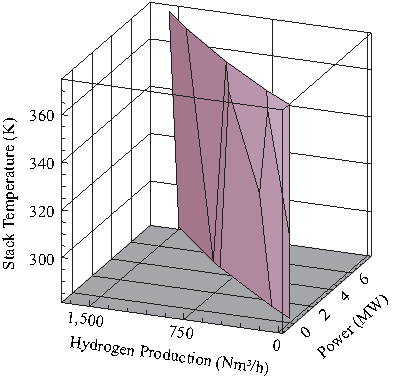
\includegraphics[scale=0.90]{dd}\vspace{-6pt}
	\caption{Polyhedral approximation of the production function of a 1,000 Nm$^3$/h-rated stack.}
	\label{fig:dd}
\end{figure}

\subsubsection{Reduced-Order Approximation of the HTO Accumulation Process}
\label{sec:htosimply}

As discussed in Section \ref{sec:hto}, the process of HTO accumulation takes three stages. % in the anode half-cell, the liquid phase of the separator, and the gas phase of the separator.
%Among these, 
The time constants for the anode half-cell and liquid phase of the separator are on the orders of seconds and minutes, while the gas-phase time constant ranges to tens of minutes. Thus, we can focus solely on the gas phase and adopt a first-order model to approximate the entire process:
\begin{align}
  \dfrac{\text{d} n^{\text{H}_2,\text{sep}}_{\text{gas}}}{\text{d}t} = \sum\nolimits_{i=1}^N \dot{n}^{\text{H}_2,\text{im}}_{i} - \dot{n}^{\text{H}_2}_{\text{out}}. \label{eq:htosimple}
\end{align}

Replacing (\ref{eq:Nbalance}) with (\ref{eq:htosimple}), the order of the model is reduced from $N$+2 to 1, improving both computational efficiency and numerical stability. Additionally, the molar quantity of HTO impurities in the half-cells and liquid phase, $ n^{\text{H}_2,\text{an}}_i$ and $n^{\text{H}_2,\text{sep}}_\text{liq}$, cannot be measured. After simplification, these variables are omitted, with the remaining $n^{\text{H}_2,\text{sep}}_\text{gas}$ easily measurable, thereby eliminating the need for a state estimator.

\begin{remark}
%It is worth noting that the 
The time constants of the heat transfer processes among stacks, separators, and the heat exchanger do not differ by order of magnitude. Therefore, unlike the HTO process, reducing the order of the temperature dynamic model would introduce noticeable errors. This has been discussed in studies on 1-in-1 systems \cite{qi2023thermal}, and the same applies to $N$-in-1 systems.
\end{remark}


\subsubsection{Bilinear Terms in Temperature and Mass Transfer Dynamics}
\label{sec:bilinear}

The state-space model presented in Section \ref{sec:model} has bilinear terms, which cannot be relaxed as convex as in Section \ref{sec:polynomial}. To address these terms, we employ a discretization-based big-M method \cite{bemporad1999control}.

The bilinear terms requiring reformulation include $I_i T_{i,\text{s}}$, $I^2_i$, $I_i {n}_{\text{gas}}^{\text{H}_2,\text{sep}}$, $v_{i,\text{lye}} T_{i,\text{s}}$, $v_{i,\text{lye}} T_{\text{sep,out}}$, and $v_{\text{c}} T_{\text{c,out}}$. Taking $I_i T_{i,\text{s}}$ as an example, the following steps are applied. First, discretize $I_i$ as
\begin{align}
  I_i = \sum\nolimits_{k=1}^{N^\text{d}} 2^{k-1} \beta^{I}_{i,k} \Delta I,   \label{eq:idist}
\end{align}
\noindent
where $N^\text{d}$ is the number of binary bits; $\Delta I = \overline{I}/2^{k}$ is the step size; and $\beta^{I}_{i,k}$ represents the $k$th binary variable. Then, $I_i T_{i,\text{s}}$ can then be replaced with:
\begin{gather}
  I_i T_{i,\text{s}} = \sum\nolimits_{k=1}^{N^\text{d}} 2^{k-1} \delta^{I,T}_{i,k} \Delta I,   \label{eq:itdist} \\
  T_{i,\text{s}} - M \big(1- \beta^{I}_{i,k} \big) \le  \delta^{I,T}_{i,k}  \le T_{i,\text{s}} + M  \big(1- \beta^{I}_{i,k} \big), \label{eq:itbigm1} \\
  - M  \beta^{I}_{i,k}  \le  \delta^{I,T}_{i,k}  \le M  \beta^{I}_{i,k} , \label{eq:itbigm2}
\end{gather}
where $\delta^{I,T}_{i,k}$ is an intermediate variable; $M$ is a sufficiently large constant. This reformulation converts bilinear terms into mixed-integer linear constraints, which can be efficiently solved using commercial solvers.
%Detailed descriptions of the big-M method can be found in classical literature such as \cite{bemporad1999control}.

\subsubsection{Controller Summary}
\label{sec:controlsummary}

After the aforementioned simplification, the optimization model in the NMPC is transformed as a mixed-integer quadratic programming (MIQP) problem, expressed compactly as:
\begin{align}
  \max\ (\ref{eq:obj}), \ \text{s.t.} \ (\ref{eq:diststate}), (\ref{eq:prodieq}), (\ref{eq:limitcellvolt}){\text{--}}(\ref{eq:limitcool}),(\ref{eq:idist}){\text{--}}(\ref{eq:itbigm2}).    \label{eq:mpcall}
\end{align}

%This problem can be directly solved using commercial solvers such as Gurobi.
%Furthermore,
%Due to the simplifications applied to the model, and considering the reduced dynamic time constants of the temperature and HTO models (on the order of tens of minutes),
With the simplified model, we can set a control horizon ranging from a few minutes to an hour, and the step length to several minutes. %, and the
Under these conditions, solving the NMPC takes only a few seconds, meeting real-time operation requirements.

During implementation, as in standard MPC procedures, %the optimization 
(\ref{eq:mpcall}) is solved every few seconds based on the power reference and measurements of temperature and HTO impurity concentration. The first step of the obtained control series is applied. % to the AWE system. 
By repeating this process, the $N$-in-1 system dynamically allocates power among the $N$ stacks, and adjusts lye circulation and cooling water flow rates, achieving load tracking, temperature stabilization, and suppression of HTO accumulation under dynamic power input. During this process, the pressure and liquid levels are regulated by a separated controller, which is not covered in this work, as noted by Assumption A in Section \ref{sec:assumptions}.

\begin{remark}
	\label{remark:2}
	The NMPC proposed here not only targets the optimal control of $N$-in-1 systems but also aims to provide a fair ground for the performance comparison among $N$-in-1 systems with different lye distribution topologies and the 1-in-1 system, as the controller can easily adapt to different configurations by slightly modifying the integrated state-space model while preserving optimality. Leveraging it, we can answer the Question 1 raised in the Introduction; see Sections \ref{sec:comparetopo}--\ref{sec:comparemulti}.
\end{remark}

\section{Simulation Studies}
\label{sec:case}

\subsection{Simulation System Setup}
\label{sec:setting}

A 4-in-1 configuration, commonly used in real-world projects \cite{zhangalkaline,zhai2024review}, is selected for analysis. The nominal production rate of the system is set to 4,000 Nm$^3$/h, with each stack to be 1,000 Nm$^3$/h. The stack parameters are based on a test platform with a 1-in-1 configuration in \emph{Beijing Power Equipment Group in China} \cite{li2024optimization}, while the parameters of the BoP are scaled proportionally. % according to the platform. 
The parameters used in the simulation are detailed in Table \ref{tab:parameter} in Appendix A.

For the controller setup, the horizon and step length are set as $N^\text{h}=1,800$ s and $\Delta t =  450$ s. The weight coefficients in the objective function (\ref{eq:obj}) are set as $\lambda^{\text{prod}}=1$,  $ \lambda^{\text{track}}=1.2$, $\lambda^{\text{temp}}=0.15$, $\lambda^{\text{I}}=0.0002$, $ \lambda^{\text{lye}}  = 25,000$, and $ \lambda^{\text{c}} = 0.5$. The complete model presented in Section \ref{sec:model} and Table \ref{tab:model} is used for time-domain simulation, preserving all nonlinear dynamic processes. The NMPC updates the control commands every 10 seconds based on the optimization model 
summarized in Section \ref{sec:controlsummary}. % to update the control commands for electrolytic currents, lye circulation rates, and cooling water flow rate.
Simulations are performed on \emph{Wolfram Mathematica 13.0}, and the optimization problem in the controller is solved via \emph{Gurobi 11.0.3}.


\begin{figure}[tb]
	\centering
	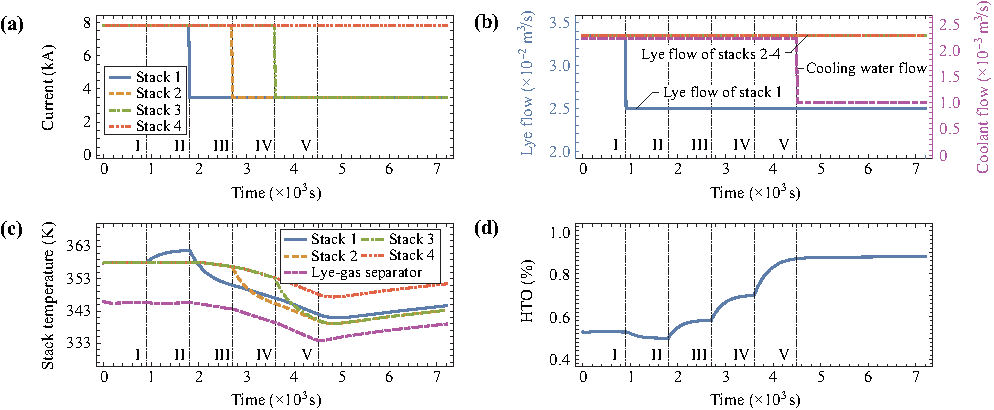
\includegraphics[scale=0.9]{openloop}\vspace{-6pt}
	\caption{Open-loop responses of the 4-in-1 AWE system. (a) Electrolytic currents of the stacks. (c) Lye flow rates of the stacks and Cooling water flow rate. (c) Temperature of the stacks and separator; (d) HTO impurity at the gas phase of the separator.}
	\label{fig:openloop}
\end{figure}

\subsection{Open-Loop Simulation}
\label{sec:openloop}

An open-loop simulation is conducted without the feedback controller  %analyze the dynamic behavior of the 4-in-1 system, in order 
to demonstrate the cross-coupling relationships between control (i.e., current, lye flow rate, and cooling water flow rate) and responses (such as temperature and HTO impurity concentration), as shown in Fig. \ref{fig:state}. The system employs the 4-pump configuration shown in Fig. \ref{fig:cir}(a), allowing independent adjustment of the lye flow rate for each stack. 
The initial conditions are set as follows: stack temperature at 85 $^\circ$C (358 K), separator temperature at 73 $^\circ$C (345 K), and HTO concentration at 0.52\%. 
%The initial stack temperature is set to 85 $^\circ$C (358 K), with the separator temperature set to 73$^\circ$C (345 K), and the HTO concentration set to 0.52\%. 
The control actions for current, lye flow, and cooling water flow are plotted in Fig. \ref{fig:openloop}(a) and \ref{fig:openloop}(b).

We can observe that, at 900 s, when the lye flow rate of stack 1 steps down from $3.35 \times 10^{-2}$ m$^3$/s to $2.5 \times 10^{-2}$ m$^3$/s (Action I), the temperature of stack 1 rises while the HTO concentration decreases slightly by 0.5 K. At 1,800 s, 2,700 s, and 3,600 s, the electrolytic currents of stacks 1--3 successively step down from 7,800 A to 3,500 A (Actions II, III, and IV), which leads to temperature drops in these stacks and a gradual decline in separator temperature to 333.4 K (60.4  $^\circ$C,) while the HTO concentration increases from 0.50\% to 0.84\%. Finally, at 4,500 s, the cooling water flow rate is reduced from $2.2 \times 10^{-3}$ m$^3$/s to $1.0 \times 10^{-3}$ m$^3$/s (Action V), leading to a simultaneous temperature increase across all components, with a magnitude of 5.5 K in 2,500 s. Temperature variations directly affect cell voltages, %, and subsequently the production rate, 
electrolytic heat, %and HTO concentration, 
and other states.
The results highlight complex inter-couplings within the $N$-in-1 AWE system shown in Fig. \ref{fig:state}, emphasizing the necessity of considering MIMO characteristics in the controller design.

\begin{figure}[tb]
	\centering
	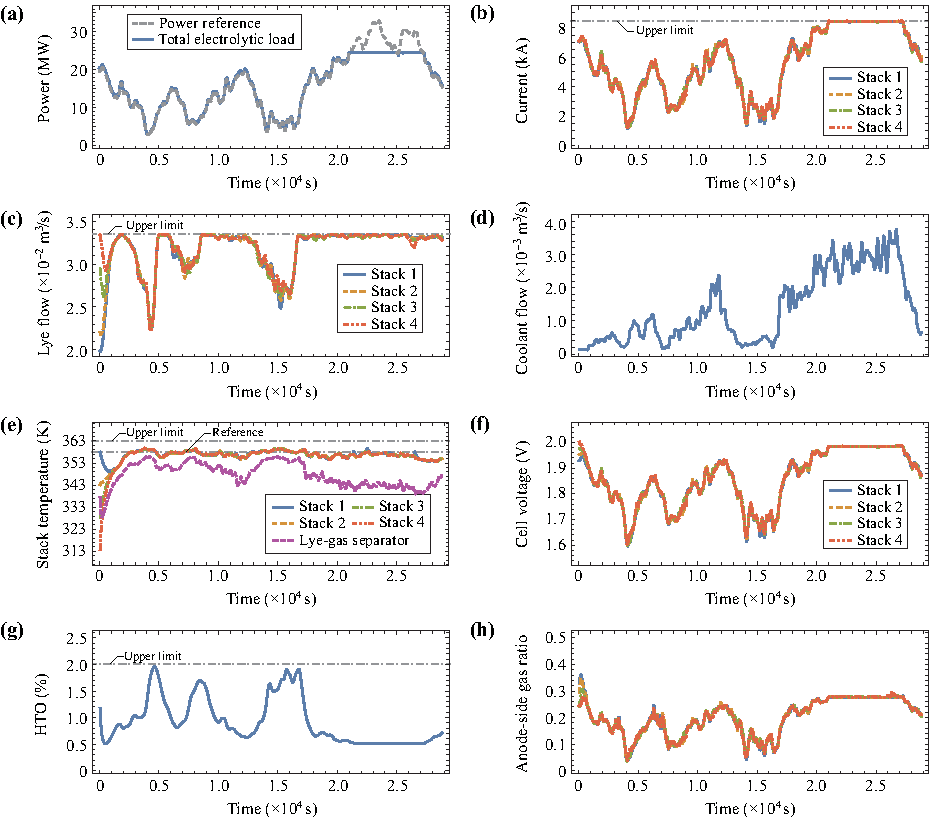
\includegraphics[scale=0.90]{4valve}\vspace{-6pt}
	\caption{Control and responses of the 4-in-1 AWE system with a 4-pump configuration. (a) Load power reference and overall power consumption. (b) Electrolytic currents of the stacks. (c) Lye flow rates  of the stacks. (d) Cooling water flow rate. (e) Temperature of the stacks and separator. (f) Cell voltage of the stacks. (g) HTO impurity at the gas phase of the separator. (h) Gas ratio in the anode half-cells.}	
	\label{fig:4valve}
\end{figure}


\subsection{Overall Performance under Dynamic Operation}
\label{sec:casebase}

The performance of the 4-in-1 system under the proposed NMPC %under varying power inputs 
is analyzed. The simulation adopts the 4-pump configuration shown in Fig. \ref{fig:cir}(a).
The load reference $P_{\text{tot}}^{\text{ref}}(t)$ emulates the fluctuations of renewable energy ranging from 6 MW to 38 MW, shown in Fig. \ref{fig:4valve}(a), and the simulation lasts for 8 hours. During the first 5 hours, the load reference fluctuates at a lower level, followed by 3 hours of high power supply, allowing a comprehensive evaluation of the dynamic operation of the AWE system.

The initial temperatures of stacks are set to 85 $^\circ$C, 70 $^\circ$C, 55 $^\circ$C, and 40 $^\circ$C (358 K, 343 K, 328 K, and 313 K), respectively. The separator temperature is set to 65 $^\circ$C (338 K), with an initial HTO concentration at 1.2\%. Throughout the simulation, the controller continuously adjusts the current, lye flow, and cooling water flow for each stack, as shown in Fig. \ref{fig:4valve}(b)--(d), and the behaviors of the 4-in-1 system are discussed.

\emph{a) Inter-stack Load Allocation:} The load is evenly shared among the 4 stacks throughout the process. This is driven by the objective function (\ref{eq:obj}), which maximizes hydrogen yield. 
As shown in Fig. \ref{fig:dd}, the relation between hydrogen yield, electrolytic power, and temperature is concave. At the point of maximum hydrogen yield, the partial derivatives of the production rate with respect to power consumption across all stacks are equal, i.e., $\partial \dot{n}_{i}^{\text{H}_2,\text{prod}} / \partial P_{i}^{\text{ele}} = \partial \dot{n}_{j}^{\text{H}_2,\text{prod}} / \partial P_{j}^{\text{ele}}$, $\forall i,j\le N$. With the stacks to be identical, this leads to an even power distribution, a phenomenon known as the \emph{equimarginal principle}, discussed in our previous work for scheduling multiple electrolyzers \cite{li2024two,zeng2024scheduling}. After 20,000 s, when the power supply exceeds the rectifiers' total power limit, i.e., 24 MW, all stacks operate at full load, saturating hydrogen production rates.

\emph{b) Temperature Dynamics:} %From the perspective of temperature control,
Due to interconnection via the BoP, heat exchange occurs between the stacks, % Therefore,
stack temperatures quickly reach uniformity at the setpoint, 85 C$^\circ$. As shown in Figs. \ref{fig:4valve}(c) and \ref{fig:4valve}(e), stacks 4 and 3, initially cooler than the separator, increase their lye flow rates to accelerate heating, while stacks 1 and 2 reduce lye flow rates to minimize heat loss. The lowermost flow rates for stacks 1 and 2 reach 0.0195 m$^3$/s and 0.0218 m$^3$/s compared to the rated value of 0.0345 m$^3$/h. Heat exchange rapidly makes stack temperatures reach unison during startup. % phase. %, optimizing the production rate.
%Fig. \ref{fig:4valve}(e) shows the temperature differences between the stacks and the separator. The controller focuses on stabilizing the stack outlet temperature, resulting in the largest temperature differences during high-load periods, particularly after 20,000 s when all stacks operate at full load. 
%The inlet temperature is reduced by increasing cooling water flow to manage rising outlet temperatures, as shown in Fig. \ref{fig:4valve}(d). 
For the rest of the time, lye flow adjustments are minimized to avoid excessive fluctuations that could affect the gas-liquid ratio, %, except the startup phase when balancing stack temperatures is critical. 
and temperature control mainly relies on cooling water adjustments, %as shown in Fig. \ref{fig:4valve}(d),
making the stack temperature stay within a range of [81, 86] C$^\circ$.

%However, there are exceptions, such as during the period around 27,000 s, where the load reference decreases, slightly reducing the lye circulation flow to complement the cooling water flow control and prevent a rapid temperature drop in the stacks.

\emph{c) HTO Accumulation Dynamics:} Since HTO impurity concentration is not included in the objective (\ref{eq:obj}) but in the inequality constraints, the fluctuations in HTO impurity do not affect the control actions in most cases. 
However, during significant load drops (e.g., at 4,000 s, 8,000 s, and 15,000 s), the HTO concentration rises rapidly, which is similar to 1-in-1 systems. 
To prevent exceeding the safety limit 2\%, the controller reduces lye flow rates to $0.0225$ m$^3$/s, $0.0285$ m$^3$/s, and $0.0250$ m$^3$/s (67\%, 85\%, and 75\% of the rated value) respectively, mitigating lye circulation-induced HTO cross-mixing, which is modeled by (\ref{eq:nlye}). Elsewhere, to stabilize the gas-liquid ratio, the lye flow is kept near its rated value, as shown in Fig. \ref{fig:4valve}(f).

These results demonstrate that despite that the hydrogen yield, temperature, and HTO concentration are tightly coupled in the $N$-in-1 system, as shown in Fig. \ref{fig:state} and exemplified in Section \ref{sec:openloop},
%The main response variables and control inputs exhibit MIMO characteristics, with complex interdependencies and opposing control actions, as shown in Fig. \ref{fig:state}. This underscores the necessity of considering MIMO control for $N$-in-1 systems, which, although more complex than 1-in-1 systems, can be effectively managed using 
the proposed controller can manage these complexities effectively, thereby answering Question 2 posed in Section \ref{sec:motivation}.


\subsection{Comparisons Between Different Lye Circulation Topologies}
\label{sec:comparetopo}

\begin{figure}[tb]
	\centering
	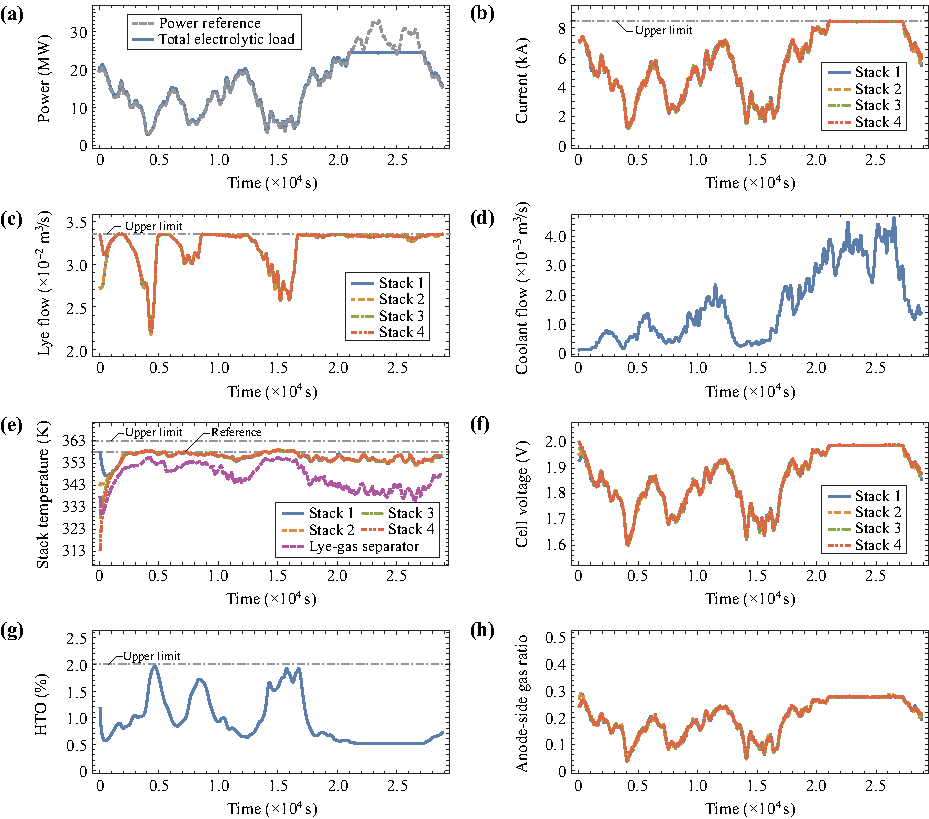
\includegraphics[scale=0.9]{2valve}\vspace{-6pt}
	\caption{Control and responses of the 4-in-1 AWE system with a 2-pump configuration shown in Fig. \ref{fig:cir}(b). (a) Load power reference and overall power consumption. (b) Electrolytic currents of the stacks. (c) Lye flow rates  of the stacks. (d) Cooling water flow rate. (e) Temperature of the stacks and separator; (f) Cell voltage of the stacks. (g) HTO impurity at the gas phase of the separator. (h) Gas ratio in the anode half-cells.}
	\label{fig:2valve}
\end{figure}

\begin{figure}[tb]
	\centering
	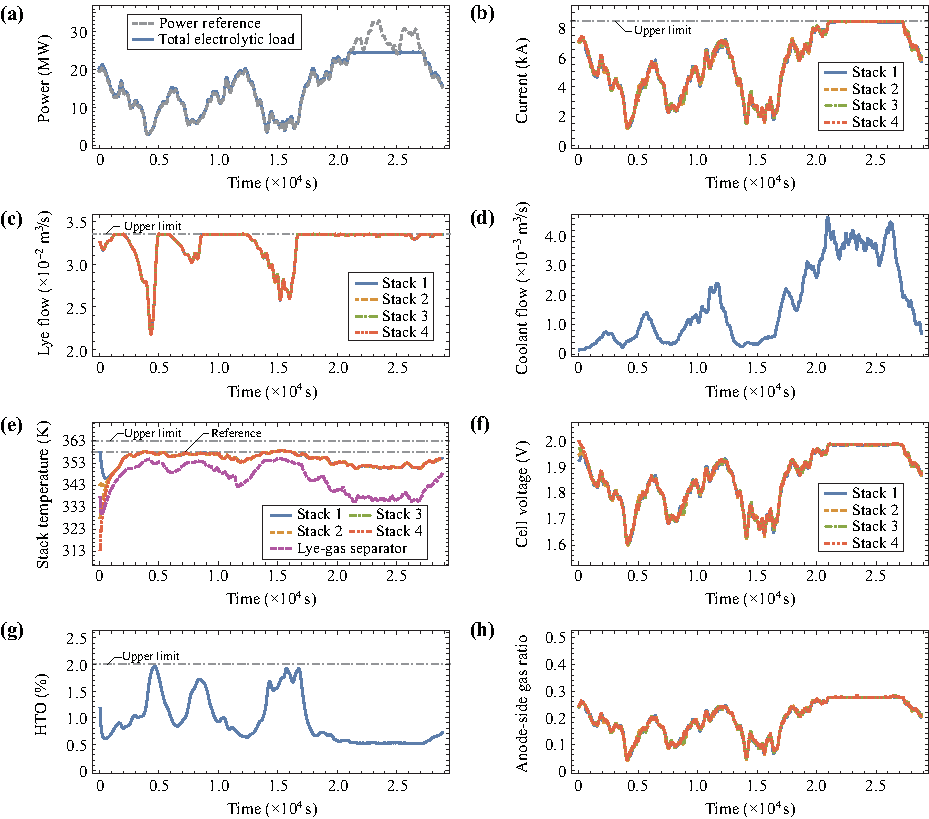
\includegraphics[scale=0.9]{1valve}\vspace{-6pt}
	\caption{Control and responses of the 4-in-1 AWE system with a 1-pump configuration shown in Fig. \ref{fig:cir}(c). (a) Load power reference and overall power consumption. (b) Electrolytic currents of the stacks. (c) Lye flow rates  of the stacks. (d) Cooling water flow rate. (e) Temperature of the stacks and separator; (f) Cell voltage of the stacks. (g) HTO impurity at the gas phase of the separator. (h) Gas ratio in the anode half-cells.}
	\label{fig:1valve}
\end{figure}

\begin{figure}[tb]
	\centering
	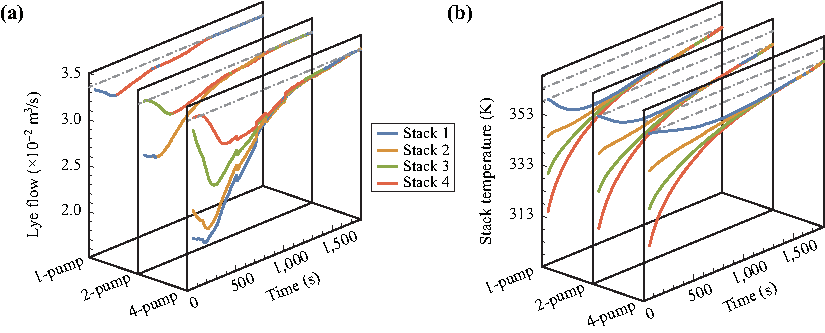
\includegraphics[scale=0.9]{compcirs}\vspace{-6pt}
	\caption{Comparison on control and responses of the 4-in-1 AWE system with 1-pump, 2-pump, and 4-pump configurations. (a) Lye flow rates  of the stacks. (b) Temperature of the stacks.}
	\label{fig:compcir}
\end{figure}

%\begin{table}[tb]\scriptsize\centering
%	\renewcommand{\arraystretch}{1.45}
%	\caption{Performance comparison between 4-in-1 AWE systems with different lye circulation topologies and four 1-in-1 systems operating in parallel}\vspace{6pt}
%	\label{tab:compare}
%	\begin{tabular}{ ccccccc }\hline\hline
%		Configuration & \tabincell{c}{Energy use\\(MWh)}   & \tabincell{c}{Load-tracking\\RMSE (MW)} & \tabincell{c}{Load-tracking \\ RMSE for first \\  5 hours (MW)}                & \tabincell{c}{RMSE for stack \\   temperature  \\control (K)} &  \tabincell{c}{Total hydrogen \\ yield (Nm$^3$) }  &  \tabincell{c}{Specific energy \\consumption \\(kWh/Nm$^3$) } \\ \hline
%		4-in-1 (4-pump)   & 126.602   & 2.070     & 0.382     & 3.326     & 22,869.8   & 5.536 \\
%		4-in-1 (2-pump)   & 126.728   & 2.057     & 0.391     & 2.894     & 22,873.5   & 5.540 \\
%		4-in-1 (1-pump)   & 126.790   & 2.051     & 0.394     & 3.036     & 22,873.3   & 5.543 \\ \hline
%		Four 1-in-1 systems  & 126.702   & 2.073     & 0.394     & 2.237     & 22,879.8   & 5.538 \\ \hline\hline
%	\end{tabular}
%\end{table}

\begin{table}[tb]\scriptsize\centering
	\renewcommand{\arraystretch}{1.45}
	\caption{Performance comparison between 4-in-1 AWE systems with different lye circulation topologies and four 1-in-1 systems operating in parallel}\vspace{6pt}
	\label{tab:compare}
	\begin{tabular}{ ccccccc }\hline\hline
		Configuration & \tabincell{c}{Energy use\\(MWh)}   & \tabincell{c}{Load-tracking\\RMSE (MW)} & \tabincell{c}{Load-tracking \\ RMSE for first \\  5 hours (MW)}                & \tabincell{c}{RMSE for stack \\   temperature  \\control (K)} &  \tabincell{c}{Total hydrogen \\ yield (Nm$^3$) }  &  \tabincell{c}{Specific energy \\consumption \\(kWh/Nm$^3$) } \\ \hline
		4-in-1 (4-pump)       & 124.495   & 2.151	  & 0.379	  & 3.599   & 24,007.2  & 5.186 \\
		4-in-1 (2-pump)       & 124.521	  & 2.148     & 0.379	  & 4.055   & 23,997.9	& 5.189 \\
		4-in-1 (1-pump)       & 124.528	  & 2.149	  & 0.381	  & 5.502	& 23,977.4	& 5.193 \\ \hline
		Four 1-in-1 systems   & 124.482	  & 2.159	  & 0.376	  & 2.237	& 24,000.4	& 5.186 \\ \hline\hline
	\end{tabular}
\end{table}

As discussed in Section \ref{sec:lye}, the degree of freedom in controlling lye flow distribution varies across different topologies. To evaluate their impact on the performance of the AWE system under varying loads, this section performs simulations with the three topologies in Fig. \ref{fig:cir}, using the load power reference shown in Fig. \ref{fig:4valve}(a). All other parameters of the AWE system and controller remain constant. 

Figs. \ref{fig:2valve} and \ref{fig:1valve} present the 8-hour simulation results for the 2-pump and 1-pump configurations, respectively. Apart from the differences in inter-stack lye flow distribution during the startup phase, the control commands for electrolytic current, cooling water flow, and performance metrics (including load tracking, temperature stabilization, and suppression of HTO concentration) are nearly identical across all configurations, with no significant differences observed.

To further analyze the transient behavior of AWE systems with different topologies, the control of lye flow and the temperature responses during the first 30 minutes are shown in Fig. \ref{fig:compcir}. % We can observe differences in lye flow control among the topologies. 
In the 4-pump topology, lye flow rates in the stacks decrease by large and differing levels first and rise afterward, as analyzed in Section \ref{sec:casebase}. 
In contrast, in the 2-pump and 1-pump configurations, stacks sharing a common circulation pump exhibit nearly identical lye flow rates, which cannot be independently adjusted, as noted in Section \ref{sec:lye} and Remark \ref{remark:1}. Therefore, these systems cannot actively regulate inter-stack heat exchange through differential lye flow, and the controller instead maintains higher lye flow rates (higher than 0.0272 m$^3$/s and 0.0318 m$^3$/s for the 2-pump and 1-pump configurations, respectively) across all stacks to accelerate the process of reaching temperature unison.
%, accelerating the overall thermal circulation to balance the temperatures across the system.

As a result, the temperatures of stacks 1 and 2 in the 2-pump and 1-pump configurations drop significantly (10.5 K and 12 K for stack 1 in the 2-pump and 1-pump systems), reducing energy conversion efficiency. In the 4-pump configuration, however, the temperature drops for stacks 1 and 2 are mitigated (8.5 K for stack 1) due to independent lye flow control. %, which allows faster adaptation to initial temperature differences. 
After the startup phase, temperatures across all four stacks in all configurations converge at the setpoint $85$ C$^\circ$, and lye flow rates return to their rated values. From this point on, as shown in Figs. \ref{fig:4valve}, \ref{fig:2valve}, and \ref{fig:1valve}, there are no significant differences.

These results highlight that differences in lye circulation topology can lead to notable variations in transient characteristics. % for $N$-in-1 AWE systems. 
Nevertheless, the proposed NMPC effectively accommodates these differing characteristics by optimizing multiple control actions from a global perspective, achieving similar performances.

Table \ref{tab:compare} summarizes key performance metrics, including the electricity consumption, hydrogen yield, load tracking deviation, and energy consumption over the entire 8-hour simulation. Due to the reduced control flexibility in the 2-pump and 1-pump configurations, %lye flow rate adjustments are slightly constrained during rapid transients, 
we can observe slight increases in the temperature control RMSE by $0.456$ and $1.903$ K and marginal increases in specific energy consumption by 0.003 and 0.007 kWh/Nm$^3$, respectively, compared to the 4-pump configuration. Nevertheless, as the proposed controller can adapt %s lye flow rates % and current distribution 
to varying conditions, the absolute differences in the metrics are minimal, and the relative differences are less than $0.13$\%, which may not be noticeable in the application.
In conclusion, under reasonable control, the impact of lye circulation topology on overall performance is negligible.

\subsection{Comparing the $N$-in-1 System with Multiple 1-in-1 AWE Systems}
\label{sec:compare1in1}

\begin{figure}[tb]
	\centering
	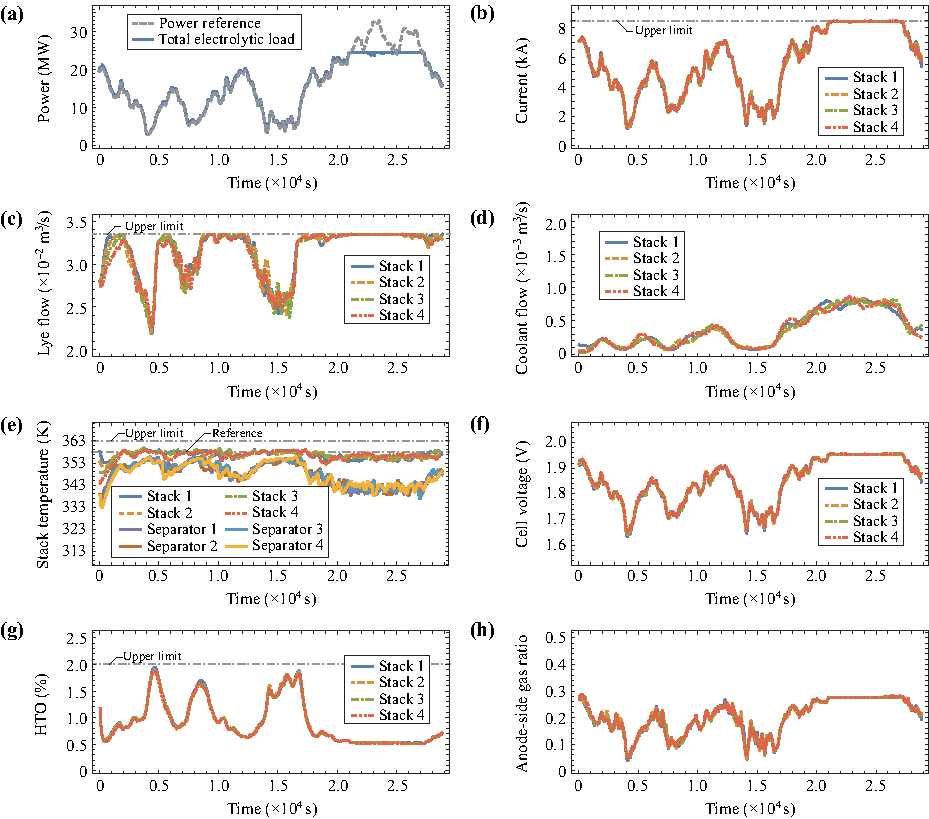
\includegraphics[scale=0.9]{four1in1}\vspace{-6pt}
	\caption{Control and responses of four traditional 1-in-1 AWE systems operating in parallel. (a) Load power reference and overall power consumption. (b) Electrolytic currents of the stacks. (c) Lye flow rates of the stacks. (d) Cooling waters flow rate. (e) Temperature of the stacks and separators; (f) Cell voltage of the stacks. (g) HTO impurity at gas phase of the separator. (h) Gas ratio in the anode half-cells.}
	\label{fig:four1in1}
\end{figure}

\begin{figure}[tb]
	\centering
	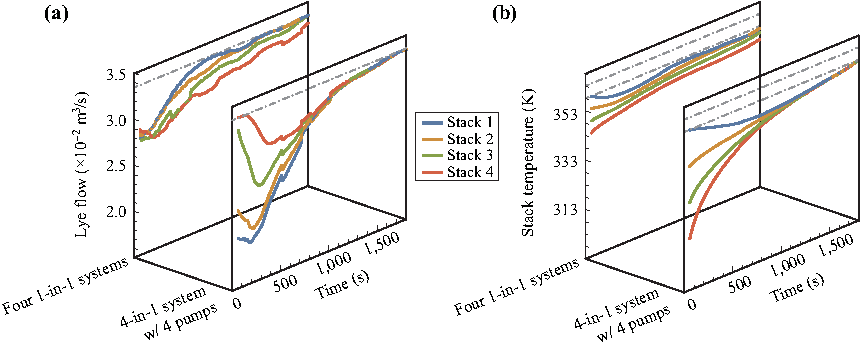
\includegraphics[scale=0.9]{comp1in1}\vspace{-6pt}
	\caption{Comparison on control and responses between the 4-in-1 AWE system with a 4-pump configuration and four traditional 1-in-1 system in parallel. (a) Lye flow rates  of the stacks. (b) Temperature of the stacks.}
	\label{fig:comp1in1}
\end{figure}

Considering the Question (a) posed Section \ref{sec:motivation}, while many ReP2H projects have invested in $N$-in-1 AWE systems, academic research has predominantly focused on 1-in-1 systems. To fill this gap, it is essential to analyze the differences between these two configurations in terms of flexibility, energy efficiency, and other aspects. This section conducts a comparative study to address these differences.

The 4-in-1 system with a 4,000 Nm$^3$/h-rated capacity, as described in Section \ref{sec:setting}, is compared with four 1-in-1 systems operating in parallel, each with a 1,000 Nm$^3$/h rated capacity, given the load reference signal shown in Fig. \ref{fig:4valve}(a). Parameters for the 1-in-1 systems are also based on the test platform at \emph{Beijing Power Equipment Group} \cite{li2024optimization}. The stack settings for the 1-in-1 systems are identical to those of the 4-in-1 system, with the parameters of BoP components %such as separators and heat exchangers 
scaled proportionally to 
$1/N$ of the 4-in-1 system. For a fair comparison, the 1-in-1 systems are also controlled using the proposed NMPC, with $N$ set to 1 and other settings unchanged.
Given that AWE systems require 40 minutes to 1 hour for a full cold startup, and the focus here is on the varying-load operation, we assume that all four 1-in-1 systems remain in operation. Startup and shutdown scheduling is excluded and left for future studies.

As in Section \ref{sec:casebase}, the initial temperatures of the stacks in the 1-in-1 systems are set to 85~$^\circ$C, 70~$^\circ$C, 55~$^\circ$C, and 40~$^\circ$C, respectively, with the initial temperature of the separators to be 65 $^\circ$C, and the initial HTO concentration at 1.2\%. 
Fig. \ref{fig:four1in1} presents the simulation results for the four 1-in-1 systems, while Fig. \ref{fig:comp1in1} compares the lye flow control and temperature responses during the initial phase.

By comparing the results of the 4-in-1 system in Sections \ref{sec:casebase} and \ref{sec:comparetopo} with the 1-in-1 systems, we can find that the behaviors of the two configurations are largely similar. As discussed in Section \ref{sec:casebase}, under the equimarginal principle, stacks evenly share power to maximize hydrogen production. In the 1-in-1 systems, the independence of temperature and lye flow control leads to nearly identical control actions under the same objectives.

A minor difference arises during the initial phase due to the absence of inter-stack heat exchange in the 1-in-1 systems. As shown in Fig. \ref{fig:comp1in1}, the lack of differential lye flow control for temperature equalization results in gentler control actions for lye flow and temperature in the 1-in-1 systems. For the 4-in-1 system, the stack lye flow rates drop by 33\% at most to 0.225 m$^3$/s, while for the 1-in-1 systems the maximal drop is by 18.5\% to 0.273 m$^3$/s . However, as stack temperatures converge, these differences decay, though the stack temperatures in 1-in-1 system converge in a slower manner due to heat insulation among the stacks.

The performance metrics summarized in Table \ref{tab:compare} also show that the efficiency, load-tracking performance, and other key indicators are nearly identical between the two configurations. The differences in load-tracking RMSE, stack temperature RMSE, and specific energy consumption are less than $0.010$ MW, $3.265$ K, and $0.007$ kWh/Nm$^3$ even for the 1-pump configuration. This similarity suggests that the 4-in-1 system and 1-in-1 systems are interchangeable from a dynamic performance perspective. Therefore, as the answer to Question 1, employing the 4-in-1 system %to reduce costs and plant area 
does not compromise flexibility or efficiency.

It is worth noting, however, that this study assumes all stacks in the $N$-in-1 system maintain an operational state. In practice, hydrogen plants with multiple 1-in-1 systems allow individual electrolyzers to start up and shut down independently, offering greater long-term flexibility \cite{varela2021modeling,qiu2023extended,li2024two}. For 
$N$-in-1 systems, constraints such as pressure and liquid level control may limit the operating range when not all the stacks are active. Additionally, the temperature or HTO impurity accumulation dynamics with partial stacks turned on may introduce new challenges. % not addressed in this study.
These issues warrant further investigation. 
% but are beyond the scope of this paper, and we will not go further.


%\subsection{Parameter Sensitivity Analysis}
%\label{sec:sensitivity}


\subsection{Comprehensive Comparisons under Various Scenarios}
\label{sec:comparemulti}

Finally, to comprehensively compare the $N$-in-1 and 1-in-1 configurations, simulations were conducted under 25 wind power supply scenarios. Each scenario, lasting 8 hours and shown in Fig. \ref{fig:wind}, is based on data from an offshore wind farm collected by Ris{\o} \cite{zhang2014wind}. For each scenario, performance metrics, including total energy use, load-tracking RMSE, stack temperature control RMSE, total hydrogen yield, and specific energy consumption, are compared in Fig. \ref{fig:multi}. The average metrics are summarized in Table \ref{tab:multi}.

\begin{figure}[tb]
	\centering
	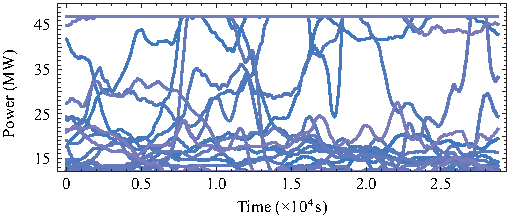
\includegraphics[scale=0.9]{wind}\vspace{-6pt}
	\caption{reference signals based on a wind farm by the Ris{\o}e }
	\label{fig:wind}
\end{figure}

\begin{figure}[tb]
	\centering
	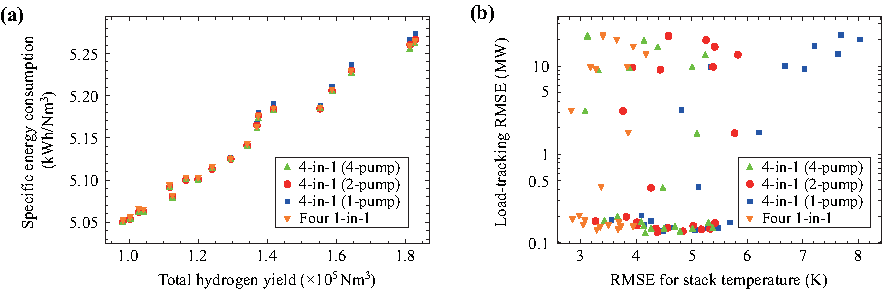
\includegraphics[scale=0.9]{multi}\vspace{-6pt}
	\caption{performance metrics of the 4-in-1 AWE systems with different lye circulation topologies and four 1-in-1 systems operating in parallel under 25 scenarios of wind power supply. (a)  Total hydrogen yield and specific energy consumption. (b) RMSE for stack temperature and load-tracking RMSE.}
	\label{fig:multi}
\end{figure}

\begin{table}[tb]\scriptsize\centering
	\renewcommand{\arraystretch}{1.4}
	\caption{Average performance metrics of the 4-in-1 AWE systems with different lye circulation topologies and four 1-in-1 systems operating in parallel under 25 scenarios of wind power supply}\vspace{6pt}
	\label{tab:multi}
	\begin{tabular}{ cccccc }\hline\hline
		Configuration & \tabincell{c}{Energy use\\(MWh)}   & \tabincell{c}{Load-tracking\\RMSE (MW)}         & \tabincell{c}{RMSE for stack \\   temperature control (K)} &  \tabincell{c}{Total hydrogen \\ yield (Nm$^3$) }  &  \tabincell{c}{Specific energy \\consumption (kWh/Nm$^3$) } \\ \hline
		4-in-1 (4-pump)       & 143.470   & 7.037	  & 4.186   & 27,674.8  & 5.165 \\
		4-in-1 (2-pump)       & 143.495	  & 7.030     & 4.667   & 27,670.0	&  5.167 \\
		4-in-1 (1-pump)       & 143.493	  & 7.032	  & 5.807	& 27,649.4	& 5.170 \\ \hline
		Four 1-in-1 systems   & 143.438	  & 7.044	  & 3.451	& 27,660.5	& 5.167 \\ \hline\hline
	\end{tabular}
\end{table}

The results indicate that the performance of the 4-in-1 and 1-in-1 configurations under varying energy inputs is not significantly different, a conclusion consistent with the findings in Sections \ref{sec:comparetopo} and \ref{sec:compare1in1}. We observe that, despite different power supply levels, the energy conversion efficiency remains nearly identical. Due to the constrained degree of freedom in lye flow control, the 4-in-1 systems with 2-pump and 1-pump configurations show a slightly higher RMSE in stack temperature stabilization, leading to a marginal deterioration in energy conversion efficiency.
The average differences in load-tracking RMSE, stack temperature RMSE, and specific energy consumption are below $0.014$ MW, $2.356$ K, and $0.003$ kWh/Nm$^3$. These increases can be negligible in practical applications. %, with the figures remaining below 0.1\%. 

In summary, we answer Question 1 by confirming that selecting the 4-in-1 system does not compromise flexibility or efficiency when compared to traditional 1-in-1 systems.

\section{Conclusions}
\label{sec:conclusion}

This paper proposes a state-space model for the $N$-in-1 AWE system, considering the dynamic behaviors of lye circulation, temperature, and HTO impurity accumulation. A controller based on NMPC is developed to coordinate inter-stack electrolytic current distribution, lye flow, and cooling, ensuring the $N$-in-1 system adapts to varying energy input.

Simulations across various scenarios with fluctuating wind energy input show that, despite the increased complexity and reduced control flexibility of the $N$-in-1 system, the proposed controller design allows the $N$-in-1 configuration with different lye circulation topologies to maintain similar energy conversion efficiency and flexibility compared to independent 1-in-1 systems.

Future research may address the following aspects. This study assumes continuous operation of the AWE system throughout the simulation period. For large hydrogen plants, the scheduling of electrolyzers, including on-standby-off state switching, should be further explored, along with a plant-wise performance comparison between the $N$-in-1 and 1-in-1 configurations. Additionally, the consideration of energy input uncertainty warrants further investigation.

\section*{Acknowledgement}

The authors gratefully acknowledge the financial support from the National Key Research and Development Program of China (2021YFB4000503) and the National Natural Science Foundation of China (52377116 and 52307126).

\section*{Declaration of Interest}

None.

\section*{Data Availability}

The data related to this work are available upon request.

%\break
%\section*{Appendix A: Nomenclature}
%\label{sec:app1}
%
%\setcounter{figure}{0}
%\renewcommand{\thefigure}{A\arabic{figure}}
%\setcounter{table}{0}
%\renewcommand{\thetable}{A\arabic{table}}
%
%
%\begin{table}[h]%\footnotesize
%  \renewcommand{\arraystretch}{1}
%  \centering
%  \begin{tabular}{p{1.8cm}p{5.6cm}p{1.8cm}p{6.cm}}
%  $N^{\text{cell}}$     &   Number of cells in the stack.  & $T_{i}$           & Temperature of the $i$th HE. \\
%  $U^{\text{cell}}_i$   &   Cell voltage.                               & $T^\text{am}$, $T^\text{cool}$    & Ambient/coolant temperature. \\
%  $U^{\text{rev}}$, $U^{\text{th}}$    & Reversible/thermal neutral voltage.    & $\overline{T}$            &  Upper temperature limit. \\
%  $I_i$                 & Electrolytic current.                         & $C_i^\text{temp}$ & Heat capacity of the $i$th HE. \\
%  $\rho$                & System pressure.                              & $Q_{i}^{\text{react}}$            & Electrolytic heat. \\
%  $\eta_i^{\rm{cell}}$  & Faraday efficiency of the $i$th HE.           & $Q_{i}^{\text{diss}}$, $Q_{i}^{\text{cool}}$  & Dissipation/cooling heat. \\
%  $\dot{n}_{i}^{\text{H}_2,\text{prod}}$ & Hydrogen production flow.    & $R^{\text{diss}}$, $R^{\text{cool}}$  &  Heat resistance of dissipation/cooling. \\
%  $\dot{n}_{i}^{\text{O}_2,\text{prod}}$ & Oxygen production flow.      & $\eta^{\rm{cool}}$                & Cooling efficiency.   \\
%  $r^{\text{H}_2,\text{prod},\downarrow}$  & Lower ramping limit.       & $n_{i}^{\text{H}_2,\text{im}}$    & Moles of HTO impurity. \\
%  $r^{\text{H}_2,\text{prod},\uparrow}$    & Upper ramping limit.       & $\dot{n}_{i}^{\text{H}_2,\text{im,in}}$    & HTO impurity crossover flow. \\
%  $P_i^{\text{ele}}$    & Electrolytic power \\
%  $P_i^{\text{BoP}}$, $P_i^{\text{aux}}$   & BoP and auxiliary power. \\
%  $P_i$                 & Total power of the $i$th HE. \\
%  \end{tabular}
%\end{table}


\break
\section*{Appendix A: Parameters of the System Used in the Case Study}
\label{sec:para}

\setcounter{figure}{0}
\renewcommand{\thefigure}{A\arabic{figure}}
\setcounter{table}{0}
\renewcommand{\thetable}{A\arabic{table}}


The parameters of the 4-in-1 AWE system used for simulations in Section \ref{sec:case} are presented in Table \ref{tab:parameter}.


\begin{table}[h]\scriptsize
  \renewcommand{\arraystretch}{1.12}
  \caption{Parameters of the 4-in-1 alkaline water electrolysis system used in the simulation}\vspace{6pt}
  \label{tab:parameter}
  \centering
  \begin{tabular}{ccc}
  \hline\hline
  Parameter                                                                     & & Value                  \\  \hline
  Number of stacks $N$                                                          & & 4 \\
  Rated hydrogen production                                                     & & $4,000$ Nm$^3$/h \\
  Rated hydrogen production per stack                                           & & $1,000$ Nm$^3$/h \\
  Rated electrolytic current per stack $I^\text{norm}$                          & & 7,800 A \\
  Maximal electrolytic current per stack $\overline{I}$                         & & 1.2$\times I^\text{norm}$ \\
  Maximal stack power $\overline{P}^{\text{ele}}$                               & & $6$  MW \\
  Number of cells per stack  $N^{\text{cell}}$                                  & & $368$   \\
  Cell area $A_{\text{c}}$                                                      & & $2$ m$^2$   \\
  System pressure $\rho$                                                        & & 1.6 MPa  \\
  Differential pressure between half-cells $\Delta \rho$                        & & $0.1\% \rho$   \\
  Electrochemical parameters $r_1$, $r_2$, $r_3$, $s$                           & & $3.202\times10^{-5}$ $\Omega$, $8.970\times10^{-8}$ $\Omega$/K, $-4.193\times 10^{-12}$ $\Omega$/Pa, $7.572\times 10^{-2}$  \\
  Electrochemical parameters $t_1$, $t_2$, $t_3$                                & & $-1.070\times10^{-1}$ $\Omega$, $14.43$ $\Omega\cdot$K, $38.8$ $\Omega\cdot$K$^2$ \\
  Faraday efficiency parameters $f_1$, $f_2$                                    & & $50+ 2.5 T_s$ (A$^2$), $0.92-6.25\times10^{-6}T_s$   \\
  Upper limit of cell voltage $\overline{U}$                                    & & $2.1$ V \\
  Ramping limits $\overline{r}^{\text{H}_2,\text{prod}} / \underline{r}^{\text{H}_2,\text{prod} }$    & & $\pm 20$ Nm$^3$/(h$\cdot$s)         \\
  %Reversible voltage $U^{\text{rev}}$                                           & & $1.229$ V \\
  %Thermal neutral voltage $U^{\text{th}}$                                       & & $1.481$ V \\
  %Load ramping limits $r^{\text{H}_2,\text{prod},\uparrow}$, $r^{\text{H}_2,\text{prod},\downarrow}$  & & $\pm 1$ MW/min \\
  %Auxiliary power $P^{\text{aux}}$                                              & & 150 kW         \\
  \hline
  Ambient temperature $T_{\text{am}}$                                           & & $298$ K ($25\ ^\circ$C) \\
  Coolant temperature $T_{\text{c,in}}$                                         & & $288$ K ($15\ ^\circ$C) \\
  Stack temperature reference $T^{\text{ref}}_{\text{s,out}}$                   & & $358$ K ($85\ ^\circ$C) \\
  Stack temperature limit $\overline{T}$                                        & & $363$ K ($90\ ^\circ$C) \\
  Stack heat capacity $C_{i,\text{s}}$                                          & & $3.450\times10^7$ J/K    \\
  Separator heat capacity $C_{\text{sep}}$                                      & & $5.193\times10^7$ J/K    \\
  Heat capacity of heat exchanger $C_{\text{he}}$                               & & $2.175\times10^7$ J/K    \\
  Heat exchange area $A_{\text{c}}$                                             & & $240$ m$^2$    \\
  heat transfer coefficient $k$                                                 & & $980$ W/K$\cdot$m$^2$         \\
  Maximal cooling water flow rate $\overline{v}_\text{c}$                       & & 0.032 m$^3$/s        \\ \hline
  %Dissipation resistance $R^{\text{diss}}$                                      & & $1.2\times10^{-4}$ K/W    \\
  %Active cooling resistance $R^{\text{cool}}$                                   & & $2\times10^{-5}$ K/W    \\
  %Cooling efficiency $\eta^{\text{cool}}$                                       & & $3.98$     \\ \hline
  Anode-side half-cell lye volume $V^{\text{an}}_{i,\text{lye}}$                & & 2.5 m$^3$    \\
  Separator volume $V_{\text{sep}}$                                             & & 10.288 m$^3$    \\
  Limits of lye flow rate per stack  $\overline{v}_{\text{lye}}$, $\underline{v}_{\text{lye}}$  & & 0.0335 m$^3$/s, 0.0101 m$^3$/s    \\
  %Impurity crossover flow $\dot{n}^{\text{H}_2,\text{im},\text{in}}$            & & $0.003182$ mol/s  \\
  %Impurity discharge constant $c^{\text{im,out}}$                               & & $5.68\times10^5$ mol$^{-1}$ \\
  Thickness of the diaphragm $\delta$                                           & & 500$\times$10$^{-6}$ m \\
  Diffusion coefficient $D^{\rm{H_2}}_{\rm{eff}}$                               & & 8.569$\times$10$^{-10}$ m$^2$/s    \\
  Permeability coefficient $K^{\text{H}_2}_{\text{eff}}$                        & & 2$\times$10$^{-16}$  m$^2$   \\
  Separation time constant $\tau_\text{sep}$                                    & & $60$ s    \\
  \hline \hline
  \end{tabular}
\end{table}


%\break
%\section*{Appendix B: Simulation Results of 4-in-1 AWE Systems with Different Topologies}
%\label{sec:toporesults}
%\setcounter{figure}{0}
%\renewcommand{\thefigure}{B\arabic{figure}}
%\setcounter{table}{0}
%\renewcommand{\thetable}{B\arabic{table}}
%
%The simulation results of 4-in-1 AWE systems with 2-pump and 1-pump configurations are plotted in Fig. \ref{fig:2valve} and Fig. \ref{fig:1valve}, respectively.





\break
\section*{References}

\bibliographystyle{elsarticle-num}
\bibliography{AWE-SHAREBOP}

\end{document}




